% !TEX root = arbeit.tex
\section{Theory}
% Plain theory. Depelopments and discussion about that is part of the experiment chapter. Setup is the description of the facilities and how the test stand and measurements were setup
	Add a Chapter about electric fields?/ Basis for the simulations?
	\subsection{Requirements}
	% Mass, performance, Power consumption. (See latest references. Part of the introduction?)
	
	\subsection{Basic Theory about TOF Masspectrometry} % Allgemeine Theorie
	
	% Ionisation efficiency
	% Time focusing?
	% SNR definition. Picture?
	% Sensitivity estimation. Nessesary? If so, part of SNR discussion. Not used in the experiments explained so far...	
	
	% Priciples kann immernoch weiter ausgearbeitet werden falls nötig.
	\subsubsection{Principle} % Noch Referenzen auf Vorlesung einfügen. Evt. noch Bild eifügen von Ionen an versch. Startpositionen. Jess definitly to descibe the different scenarios and to explain which we discuss in that section.
	
	
	This chapter explains the function of a TOF instruments. A TOF mass spectrometer consists of, an ion-source, a mass analyser and a detector. The mass analyser has an ion-mirror which increases the flight distance of the ions by keeping the instrument on a certain length. A longer flight distance increases the mass resolution of the instrument.\\% Mention that later.
	In the ion source, the ions are produced. An electric field in the source is generated such that ions get trapped and focused in the centre of the source. Then ions get accelerated by applying a high voltage pulse on the extraction grid. \textcolor{red}{Include a Graphic of the IS and draw a sample electric field to explain how the extraction pulse (the door to open) works.}
	If the pulse width is long enough for all ions to leave the source during the time the pulse is applied, the ions get all the same amount of energy $W$:
	\begin{equation}
		W = \int_{0}^{s_0}q_0 E_s ds = q_0 \frac{U_0}{2}
	\end{equation}
	With $s_0$ the distance the ions get accelerated in the ion source. This distance is 1\si{\milli\metre} corresponding to half the height of the ion source. $q_0$ is the elementary charge, $E_s$ is the applied electric field strength induced by the voltage $U_0$ applied on the extraction grid.
	The ions start in centre of ionisation region and not at the grid opposite of the extraction grid. Therefore, they have the energy $q_0U_0/2$ when arriving at the extraction grid.
	This energy is equal to the kinetic energy the ions have after leaving the ion-source
	\begin{equation}
		q_0 \frac{U_0}{2} = \frac{1}{2}m v^2
	\end{equation}
	With $m$ the mass of the particle and $v$ the particle velocity. Rearranging this formula we get
	\begin{equation}
		\frac{m}{q_0} = 2 U_0\frac{t^2}{s^2}
		\label{eq:m/q}
	\end{equation}
	With $t$ the time of flight and $s$ the flight distance. Therefore, $m/q_0$ is proportional to $t^2$.\\
	
	% Discussion about the influence of the different parameters on the flight time.
	Ions starting at different positions also get a different amount of energy. Ions starting closer to the extraction grid will get less energy than ions further away from the grid. At a certain point after the source, the ions with higher energy have overtaken the slower ions. This point is at around $2\cdot s_0$ which corresponds to a very short flight distance. To shift this focal point onto to the detector, additional fields after the ion-source are applied.\\
	The ions have different thermal energies. Therefore ions of the same mass and the the same starting position will not have all the same energy when they leave the ion source. This energy spread leads to a difference in their velocity and to different flight times. This energy spread can be partially compensated by an ion-mirror (Fig.\,\ref{fig:NIMSketch}). Ions with a higher energy will penetrate deeper into the ion-mirror and have a bigger flight path than ions with less energy. Therefore, the ion-mirror is able to compensate the different start energies of the ions. % about 10% in energy spread can be compensated in this way. Search for reference of that value.
	In the worst case scenario we have one particle flying toward the extraction grid and the other particle flying with the same velocity in the opposite direction. The second particle gets decelerated and has to turn in the source. When it reached its initial position, it has the same amount of energy as the first particle. But it will always be behind the first particle by a constant time delay needed to turn around and reach its initial position. To minimize this effect, one has to minimise the distance of the ionisation region or increase the voltage of the HV pulse. A smaller ion source means less ions and therefore less signal. Increasing the HV pulse results in bigger electronic noise at the start of the spectrum and fast species such as hydrogen of helium are lost in the noise. % Evt. noch Effekte etwas besser ausführen.
	In addition, a higher HV pulse needs longer until the pulse is fully applied.
	
	% 's' is sort of a theoretical value because the velocity changes during the flight of the ions through the spectrometer.
	% Discussion about the timing 't'
	% Effect of double charged masses and where they appear. Mention why the larger instrument automatically increases the mass resolution but that due to the sizes and weight limitations of the instrument, the maximum size is give to a certain degree. Therefore, good focusing of the ions is essetiel to lower the time spread dt of the ions. Show it with reference to the corresponding equation.

	% Pulser discussion in this chapter? No, just discussion about the timings and how it works. The discussion about the fast fall time and the other parameters are part of the pulser chapter. It will be part of a repetition because of the discussion about the requirements.

	\subsubsection{Mass Calibration}
	In this section we discuss the calibration of the mass axis. According to Eq.\,\eqref{eq:m/q} the $m/q_0$ is proportional to the square of time. By rearranging Eq.\,\eqref{eq:m/q} $m$ is:
	\begin{equation}
		m = 2 q_0 U_0 \frac{t^2}{s^2}
		\label{eq:mass_Calib_pre}
	\end{equation}
	Take together all parameters which remain constant to one single constant: % Write a bit better
	\begin{equation}
		C = \frac{2 q_0 U_0 }{s^2} 
	\end{equation}
	and considering the time scale has a constant offset $t_0$, equation \eqref{eq:mass_Calib_pre} results in % Split the two ts. It is not acctually the same.
	\begin{equation}
		m = C(t-t_0)^2
		\label{eq:mass_Calib}
	\end{equation}
	In this equation there are two free parameters, $C$ and $t_0$. To calibrate a mass spectrum at least two species appearing in the spectrum have to be known to solve this equation for the two parameters.
	% [Scherer 1999]
	
	\subsubsection{Mass resolution} % Bild einfügen, wie die Mass Resolution berechnet wird.
	The mass resolution is calculated as follows. According to Eq.\ref{eq:mass_Calib} $m$ is:
	\begin{align*}
		m &= c\cdot t^2\\
		\frac{dm}{dt} &= 2ct\\
		dm &= 2ct\cdot dt\\
		\frac{m}{dm} &= \frac{ct^2}{2ct\cdot dt}
	\end{align*}
	% Source down to here is from the lecture.
	Resulting in:
	\begin{equation}
		\frac{m}{\Delta m} = \frac{t}{2 \Delta t} = \frac{\mu_t}{2 FWHM_t}
		\label{eq:mass_res}
	\end{equation}
	With $\mu_t$ the centre of the mass peak in the time domain and $FWHM_t$ the full width at half maximum. The $FWHM_t$ depends on several parameters. For example the turn around time of the particles, the energy spread resulting from different starting positions of the particles relative to the extraction grid, spread in thermal energy. The reflectron is able to compensate for the energy spread by a certain amount. % Maybe explain that a bit further
	There are also limitations of the instrument itself. For example the performance of the pulser which will be discussed later in Chap. bla.
	\begin{comment}
		Resolution limitations:
		Pulser:
		Turn around time
		Different starting positions (discussed a little bit further above)
		Reflectron: Not ideal energy focusing -> spread
		Thermic energy -> spread
		instrument limitations: not perfect pulser pulse. discussion of Pulser follows maybe a bit later.
		peak width of the single ions measured with the detector. Peak width of 1 peak is b< a factor 10 smaller than the actual peak in the mass spectrum.
	\end{comment}
	% Mass resolution is independant from the actual mass
	% Last part of the formula is from Stefans thesis.
	
	% Then continue with the calculation of the mass resolution and the calibration of the mass scale (evt. Reference further explanation how the software it acctually does (keep it short, only extend it if further nessecary)).
	
	\subsubsection{Signal-to-Noise Ratio and Sensitivity}
	
	\textbf{SNR}\\ % Write a bit more detailed. What does background corrected mean? Subtraction of the baseline if it is elevated.
	The SNR is defined as the ratio of the background corrected peak amplitude $I^{max}_P$ and the standard deviation of the base line $std(I_b)$ \cite{Agilent_TechNote_SNR}, \cite{Master_Meyer}: % Thechnical Note Agilent and Masterarbeit Stefan.
	\begin{equation}
		SNR = \frac{I^{max}_P}{std(I_b)}
		\label{eq:SNR}
	\end{equation}
	A high mass resolution improves also the signal-to-noise ratio. By better focusing the ions in the time frame, the peak gets narrower. The area under the peak corresponds to the number of ions. If the number of ions and therefore the area under the curve stays the same, a narrower peak implicates an increase in signal height and therefore in a higher SNR.\\ % In other mass spectrometers (such as sector magnets) an increase in mass resolution results in a reduction of the phase space and therefore in a loss of signal intensity.
	\\
	\textbf{Sensitivity} \\ % Really include this chapter? Because it is only an estimation of the actual performance of the instrument. If it is included, do a proper derivation of the formula!!
	The sensitivity $n_{lim}$ is the actual detection limit of the sensor. It is defined as the amount of gas detected by the instrument $n_{det}$ over the amount of ions entering the instrument $n_{p}$ times the signal intensity measured by the instrument $I_{sig}$
	\begin{equation}
		n_{lim} = \frac{n_p \cdot I_{sig}}{n_{det}}
	\end{equation}
	
	
	\begin{comment}
		SNR
		[Wells 2011]
	\end{comment}
	
	\begin{comment}
		Sensitivity
		
	\end{comment}
	
	% SNR, Sensitivity
	
	% Uncertainty cause by the 'Umkehrzeit'. Distance between 2 and 3 is always the same and depends on Uth
	
	% Include a schematics of the ion source with the different states/ effects.	
	\subsubsection{Statistical Peak Analysis}
	% See notes from the paper and make a detailed Analysis/ description of the method.
	% A/mbar alias A/ #cm^3 is a instrument specific constant. Determine it for NIM.
	

	
	\subsection{Ion Optical Design, NIM specific elements} % Inspiration from the arguments of the paper. Titel noch anpassen. Theorieteil fortlaufend hinzufügen. Ion source efficienies, reflectron double focusing, detector reflection of signal, signal matching. Density enhancement.
	% Hier das Design allgemein halten. Erst in Kapitel 'Setup' auf die Designdetails eingehen. Discuss important theory parts here and just give a short summary in the corresponding experimental parts when the theory is used.
	% Explain here as far a necessary what the function of the different subcomponents are (reflectron to increase the flight distance,...).
	
	A time of flight mass spectrometer consists of, an ion-source, a mass analyser and a detector.\\
	
	\begin{figure}[htb] % Noch schauen, ob das noch verschoben wird.
		\centering
		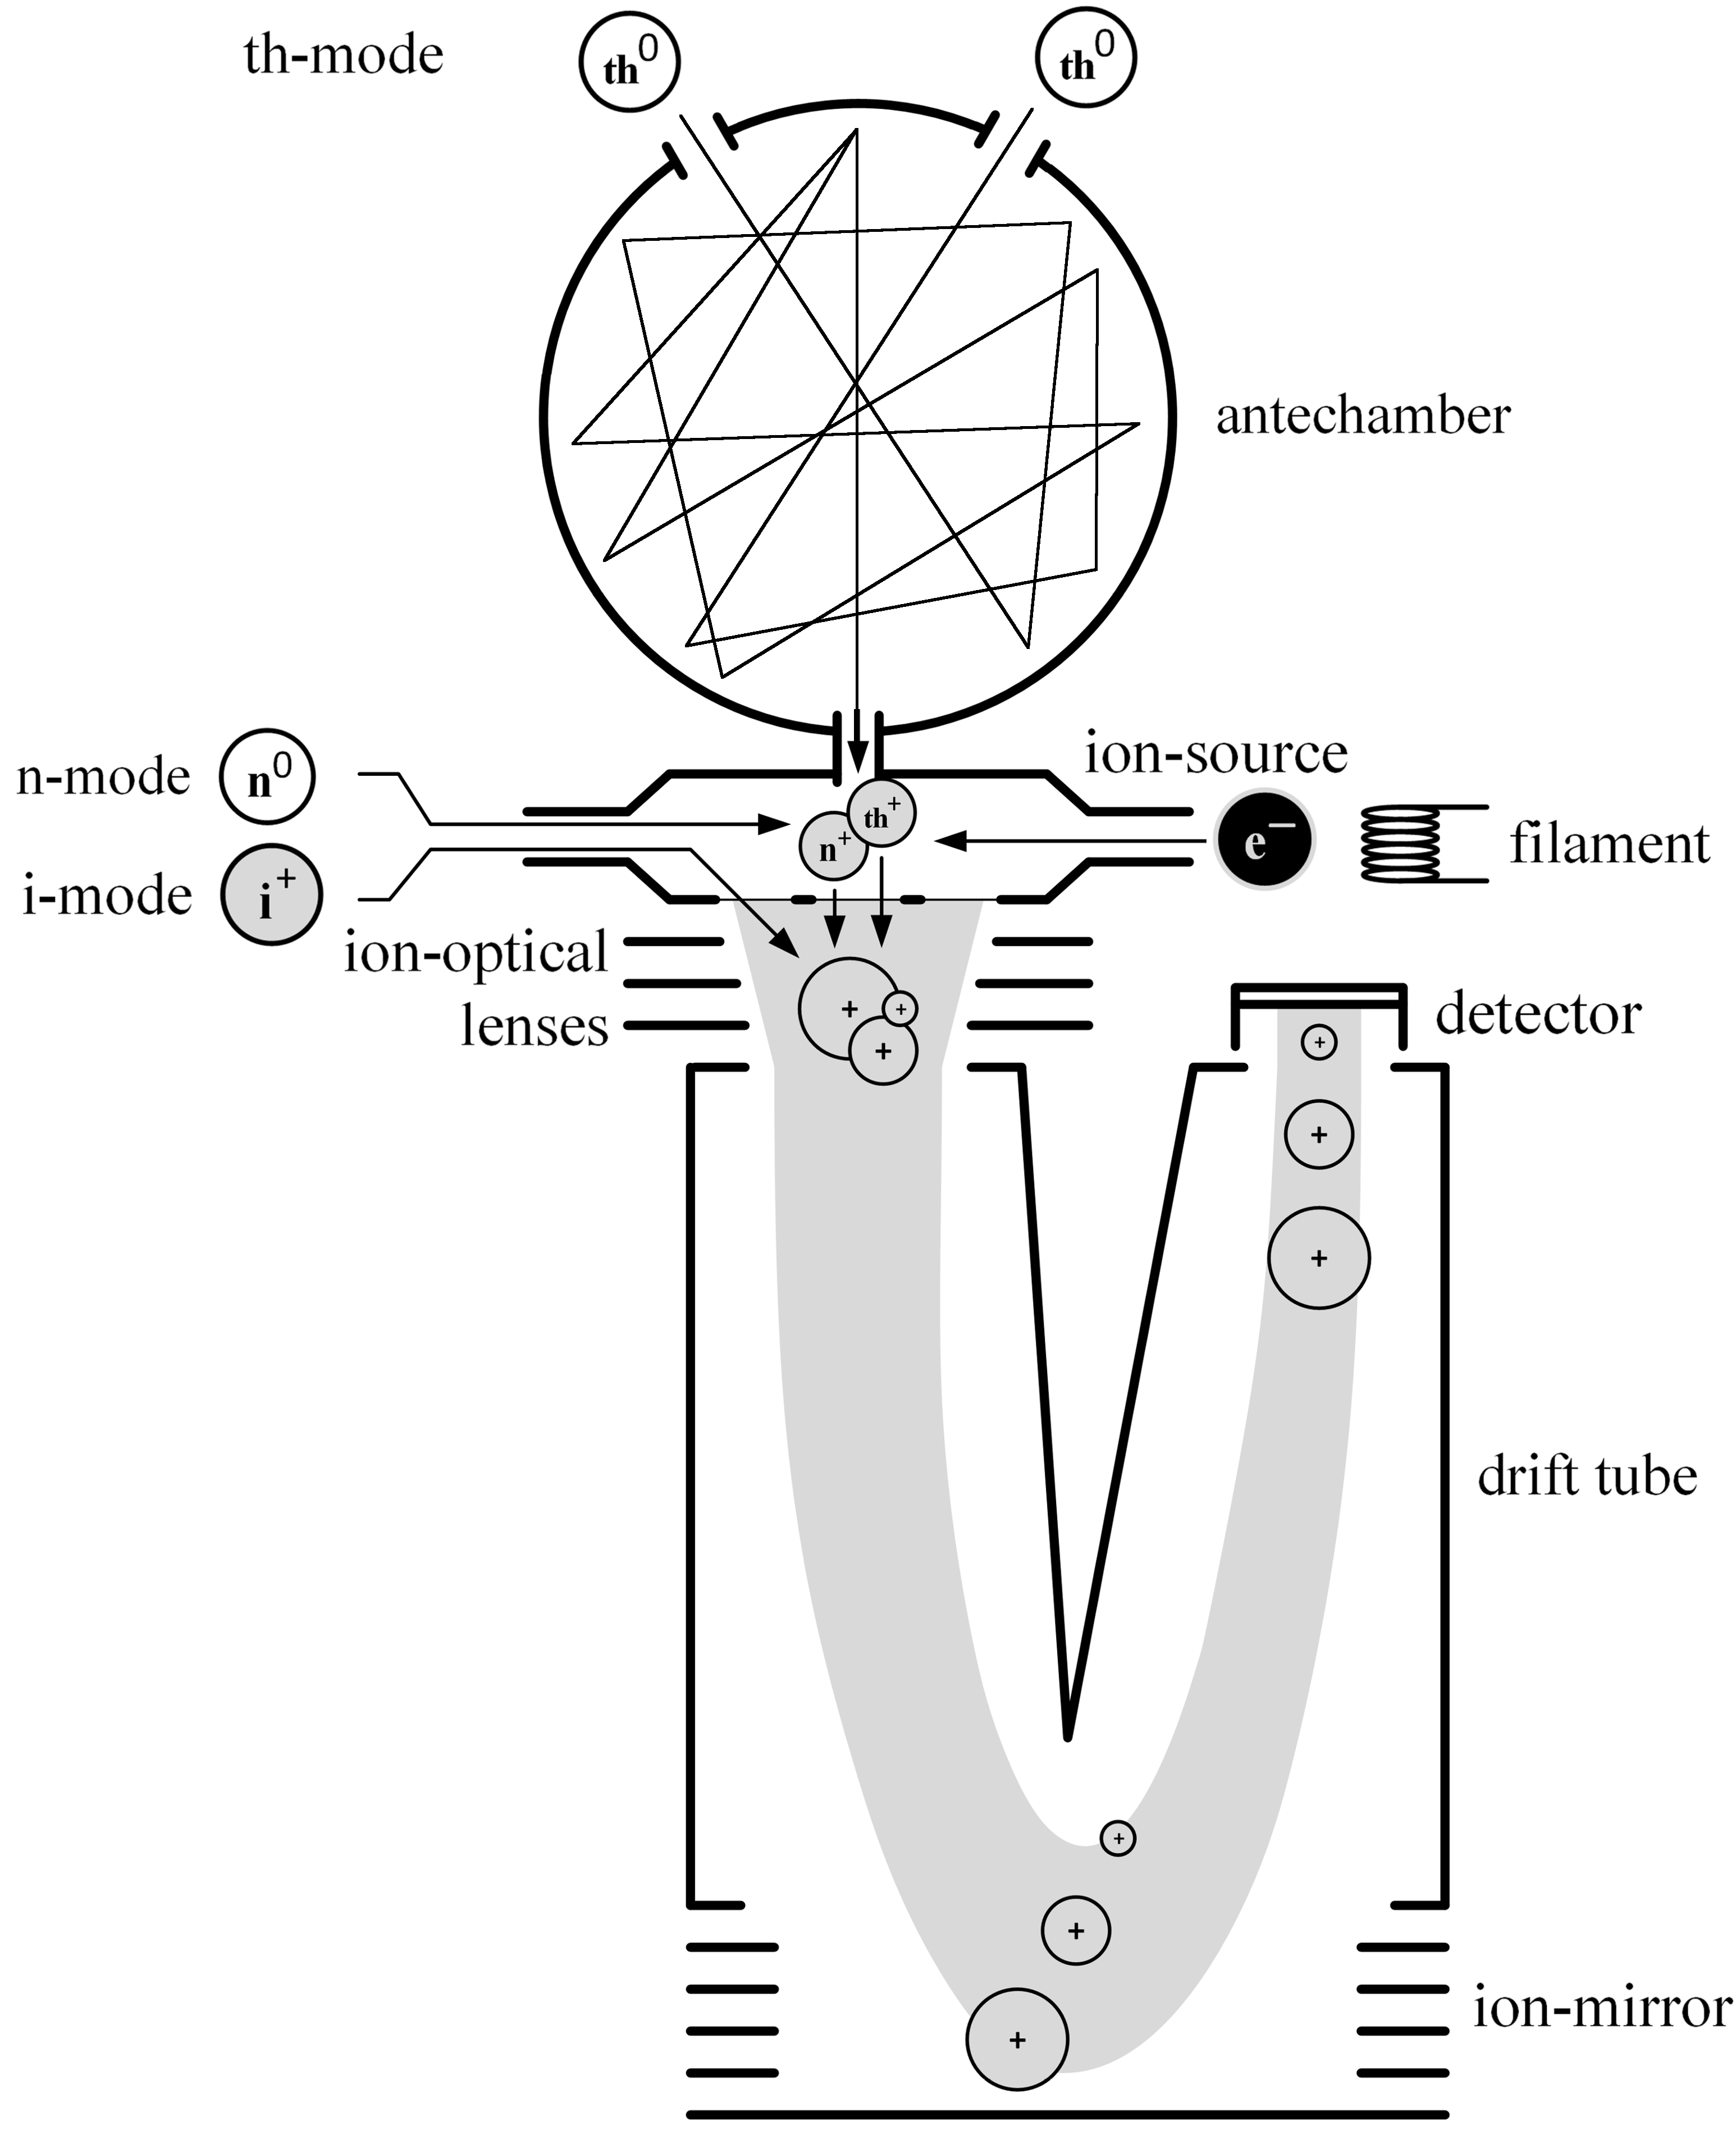
\includegraphics[width= 10cm]{Bilder/NIM_Sketch.png} % Bei Bild noch schauen, ob die Ränder drauf sind. Bei Zeiten noch Bild anpassen.
		\caption{Schematics of the NIM mass spectrometer. Adapted from \cite{Diss_Meyer}.}
		\label{fig:NIMSketch}
	\end{figure}

	%First overview and then go into the details.
	The NIM instrument is able to measure neutrals and ions. Neutral particles get ionised by electron ionisation. A filament is heated up until it emits electron. Ions enter the ion source directly.  % Noch genaue Formulierung nachschauen.
	All ions then get accelerated to the same energy and fly through the mass analyser. Light particles fly faster through the spectrometer than heavier ones. The different particle species arrive at different times at the detector. To enlarge the flight distance, an ion-mirror, which reflects the ions and leads them back to the detector. The used detector is a MCP detector. % Explain a little bit in more detail.
	
		\subsubsection{Filament Power Calculation}
		% See Diss Lukas and do the same calcultation. Make an approximation where the flight filaments should end up with the power. Do the same calculaiton also for the FS filaments. May also for the others?
		% Also mention the importance of the filament position or does it make more sense if this whole part is in the Experiment part, thus there is only an phenomenological description of the behaviour?
		% Record also of the heating current. It strongly depends on the voltage set. But maybe we see a tendency of the behaviour over time with the uncertainty factor of the voltage set. -> have a look at the data.
		
		\subsubsection{Ion Storage capability}\label{chap:IonStor}
		Ion storage of positive ions is achieved by the negative potential of the electron beam. In the following section, the potential in the centre of the electron beam is calculated. The electron emission current $I_{em}$ is:
		\begin{equation}
			I_{em} = n_e q_0 v\pi R_e^2
			\label{eq:theoElIem}
		\end{equation}
		With $n_e$ the electron volume density, $q_0$ the elementary charge, $v$ the velocity of the electrons and $R_e$ the radius of the electron beam (Fig.\ref{fig:thAntIs}). The electrons get accelerated by the negative potential applied at the filament base. This potential is around -70\,\si{\volt} resulting in a kinetic energy $U$ of 70\,\si{\electronvolt}. The velocity of the electrons is:
		\begin{equation}
			v = \sqrt{\frac{2 U}{m_e}}
			\label{eq:theoElIemVelo}
		\end{equation}
		With $m_e$ the mass of the electron. Rearranging Eq.\,\eqref{eq:theoElIem} for the volume density $n_e$ and inserting Eq.\,\eqref{eq:theoElIemVelo} for the velocity results in:
		\begin{equation}
			n_e = \frac{I_e}{q_0 \pi R_e^2}\sqrt{\frac{m_e}{2U}}						\label{eq:theoElIemNe}
		\end{equation}
		The electric field $E(r)$ in the ionization region is calculated for $R_e<r<h_{Is}/2$ with $r$ the distance from the centre of the beam and $h_{Is}$ the height of the ion source. The electric flux is defined as the surface integral of the electric field through the surface of an enclosed volume which is in this case a cylinder volume. Using Gauss's law the electric flux through the beam surface $A_{beam}$ is equal to the total charge $Q$ inside the cylinder volume.
		\begin{align}
			A_{beam} E(r) &= \frac{Q}{\epsilon_0}\\
			2\pi r l E(r) &= \pi R_e^2 l n_e q_0 \frac{1}{\epsilon_0}
		\end{align}
		Replacing the number density $n_e$ with Eq.\,\eqref{eq:theoElIemNe} and solving the equation for the electric field $E$ results in:
		\begin{equation}
			E(r) = \frac{I_e}{2 \pi \epsilon_0} \sqrt{\frac{m_e}{2U}}\frac{1}{r}
		\end{equation}
		The potential $\Phi (r)$ at a position $r$ inside of the electron beam is:
		\begin{equation}
			\Phi (r) = -\int_{h_{Is}/2}^{r} E(r') dr' = -\frac{I_e}{2\pi\epsilon_0}\sqrt{\frac{m_e}{2U}}\ln\left(\frac{R_e}{h_{Is}/2}\right)
		\end{equation}
		For calculating the electric field at a point within the electron beam at distance $0<r<R_e$ we use again Gauss's law:
		\begin{equation}
			2\pi r l E(r) = \pi r^2 l n_e q_0 \frac{1}{\epsilon_0}
		\end{equation}
		Replacing the number density $n_e$ with Eq.\,\eqref{eq:theoElIemNe} and solving the equation for the electric field $E$ results in:
		\begin{equation}
			E(r) = \frac{I_e}{2\pi\epsilon_0}\sqrt{\frac{m_e}{2U}}\frac{1}{R_e^2}
		\end{equation}
		The electric potential $\Phi (r)$ is:
		\begin{equation}
			\Phi (r) = -\int_{R_e}^{r} E(r') dr' = -\frac{1}{4\pi\epsilon_0}\sqrt{\frac{m_e}{2U}}\left(\frac{r^2}{R_e^2} -1 \right)
		\end{equation}
		And relative to border of the ion source:
		\begin{equation}
			\Phi(r) = -\frac{I_e}{4\pi\epsilon_0}\sqrt{\frac{m_e}{2U}}\left(2\ln\left(\frac{R_e}{h_{Is}/2}\right) +\frac{r^2}{R_e^2} -1 \right)
			\label{eq:elPotIem}
		\end{equation}
	
		\begin{figure}[h]
			\centering
			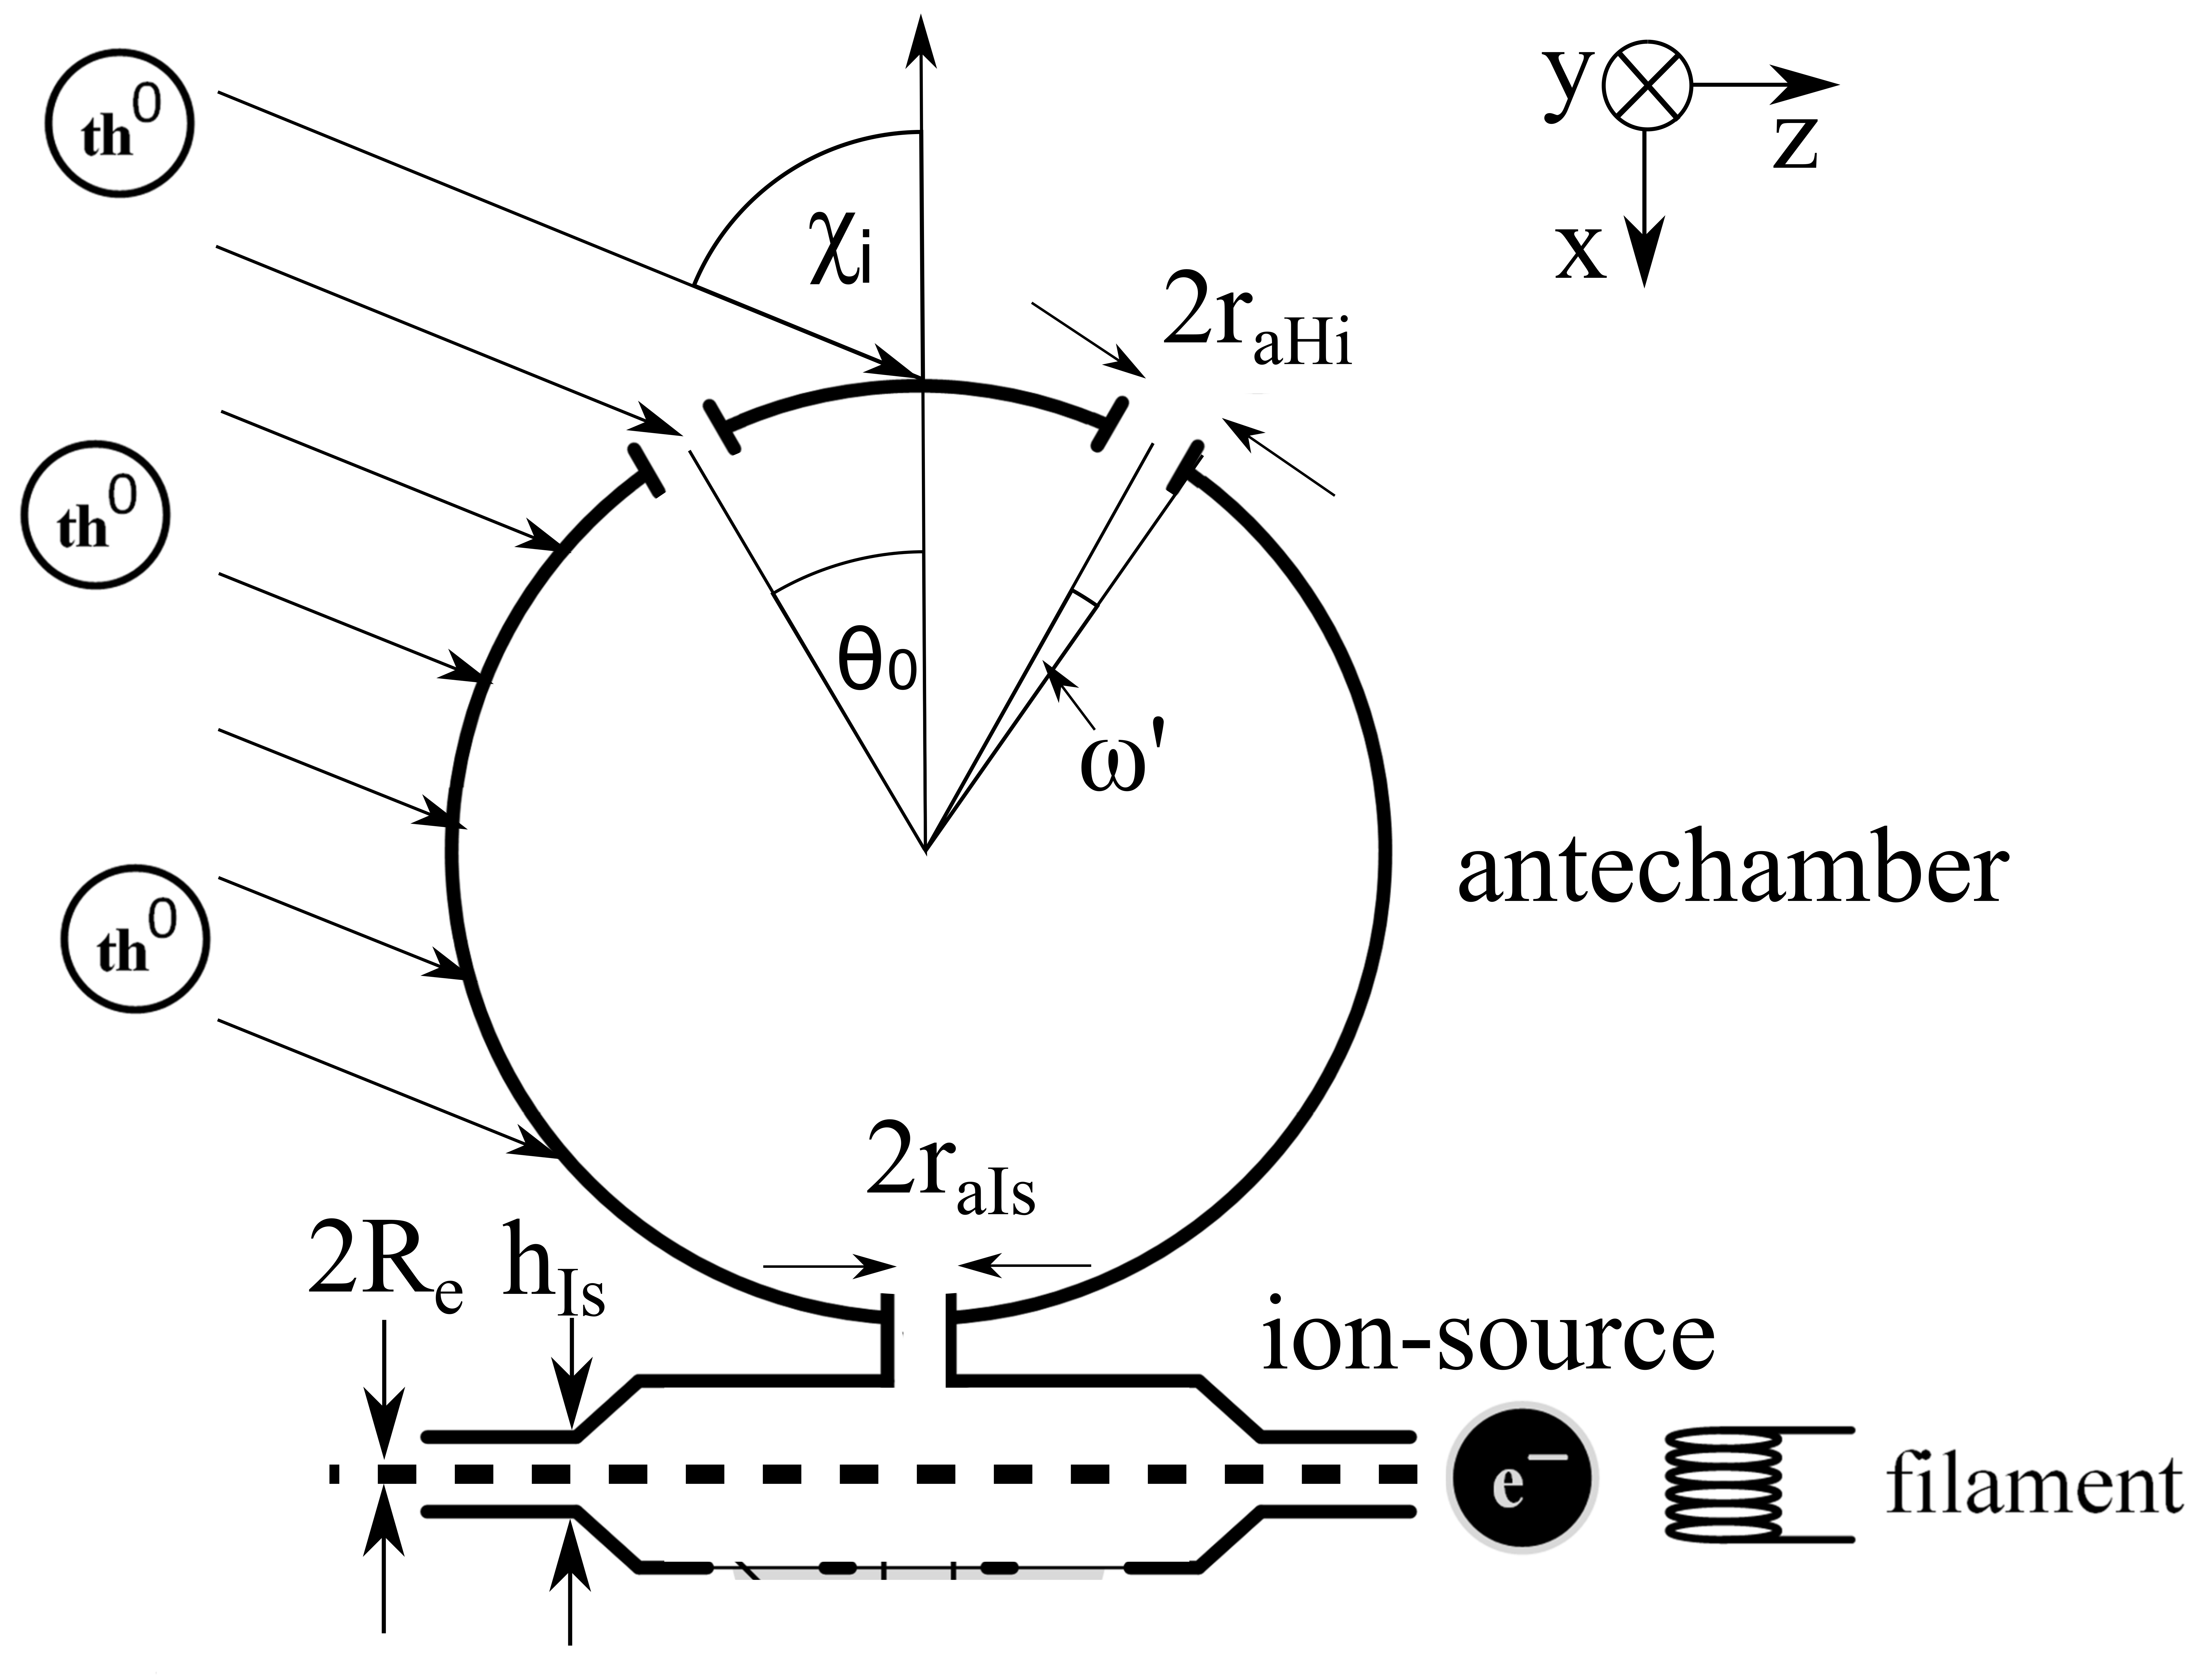
\includegraphics[width= 0.7\textwidth]{Bilder/particleDensEnh.png}
			\caption{Schematics of the antechamber and the ionisation region.}
			\label{fig:thAntIs}
		\end{figure}

%----------------------------------------------------------------------------------------------------
		\subsubsection{Density enhancement Model}\label{subsubsec:Densenhan}
		\begin{table}
			\begin{center}
				\begin{tabular}{|l r |l r |l r|}
					\hline
					$T_a$ 	& 295 K	& $r_{aHi}$	& 2.5\, mm	& $\chi$	& 0\degree \\
					$T_s$ 	& 320 K & $r_{aIs}$ & 2\, mm	& $\theta_0$& 30\degree\\	
					$k$		&	1	& $v_{sc}$	& 2.5\, km/s& $m$		& 18 u\\
					$a$		& 0.23	&			&			&			&	\\
					\hline
				\end{tabular}
			\end{center}
			\caption{Values used for the variation of the different variables of the antechamber Eq.\,\eqref{eq:thDensEnhan}.}
			\label{tab:thDensEnhan}
		\end{table}
		
		NIM has an open source entrance where neutral particles and ions enter the ionisation region directly and a closed source entrance where particles enter the ionization region after being thermalized in an antechamber. In this chapter the signal amplification factor of the closed source entrance through the antechamber is determined. The density enhancement model described in \cite{DensEnhan_Wurz_07} is used and adapted for the geometry of NIM's antechamber. The particle density $n_{cs}$ in the ionization region is:
		\begin{align}
			n_{cs} &= n_a\sqrt{\frac{T_a}{T_s}}\cdot\frac{k\cdot \sin^2\big(\frac{\omega}{2}\big)\cdot \cos^2\big(\frac{\omega}{2}\big)}{1-k\cdot \cos^2\big(\frac{\omega}{2}\big)}\frac{\big(F(S_1)+ F(S_2)\big)}{2} \frac{r_{aIs}^2\cdot a}{2\cdot r_{aHi}^2 + r_{aIs}^2\cdot a} \label{eq:thDensEnhan}\\
			F(S_i)) &= e^{-S_i^2} + \pi^{1/2}\cdot S_i\cdot\big(1 + {\rm erf}(S_i)\big) \label{eq:F(S)}
		\end{align}
		% cos(chi) = cos(theta_0)cos(theta) +- sin(theta_0)sind(theta)cos(phi)
		With $n_a$ is the particle density of the gas outside the instrument. For the tests in the laboratory $n_a$ is the particle density of then neutral gas beam, in flight it is the particle density of the moons atmosphere. In space $T_a$ is the temperature of the ambient gas and in the laboratory it is the temperature of the neutral particle beam. $T_s$ is the temperature of the antechamber. $k$ is the probability of a particle being re-emitted after colliding with the antechambers inner surface during thermalization and is close to 1 because otherwise the particles would be absorbed.\\
		$\Omega$ is the total solid angle summing up all openings through which particles enter the antechamber. NIM has two entrance holes with the same hole diameter and therefore the total solid angle $\Omega$ is the sum of the two solid angles of the entrance holes $\Omega'$:
		\begin{equation}
			\Omega = 2\cdot\Omega'
		\end{equation}
		All openings into the antechamber have a circular shape therefore, the solid angle $\Omega$ is replaced by an angle $\omega$ in the x-z-plane to simplify the equation \cite{Hedin_1964}. 
		\begin{align}
			2\pi(1- \cos(\omega)) &= 2\cdot 2\pi(1- \cos(\omega'))\\
			\cos(\omega) &= 2\cos(\omega') -1\\
			\omega &= \cos^{-1}(2\cos(\omega') -1)
		\end{align}
		$\omega'$ is the half angle of one entrance hole (Fig.\,\ref{fig:thAntIs}).\\
		$S_i$ in Eq.\,\eqref{eq:F(S)} is the speed ratio along the normal axis of the entrance hole:
		\begin{equation}
			S_i = 
			\begin{cases}
				0, & \cos(\chi \pm \theta_0) < 0\\
				v_{sc}\cdot \cos(\chi + \theta_0)\cdot \sqrt{\frac{m}{2k_B T_a}}, & i=1\\
				v_{sc}\cdot \cos(\chi - \theta_0)\cdot \sqrt{\frac{m}{2k_B T_a}}, & i=2
			\end{cases}
		\end{equation}
		with $v_{sc}$ the velocity of the neutral gas beam relative to the antechamber corresponding to the spacecraft velocity, $m$ the average particle mass of the gas and $k_B$ the Boltzmann constant. $\chi$ is the angle of the test gas relative to the x-axis of the instrument and $\theta_0$ is the angle between the x-axis and the axis normal of the entrance hole. $\chi \pm \theta_0$ is the angle between the normal axis of the entrance hole and the gas influx direction. $\chi \pm \theta_0$ has to be between $\pm 90\degree$ to enter the antechamber which implies that $\cos(\chi \pm \theta_0)$ cannot have negative values. $i=1$ is the index of one of the two entrance hole and $i=2$ is the index of the other entrance hole.\\ 
		The antechamber has three openings for the gas to flow out of the antechamber. The last term in Eq.\,\eqref{eq:thDensEnhan} gives the ratio of how many particle leave the antechamber through the hole connecting the antechamber with the ionization region compared to the amount of particles leaving the antechamber through the two entrance holes. The radius of the entrance holes is $r_{aHi}$ and the radius of the hole connecting the antechamber with the ionization region is $r_{aIs}$. This term takes the molecular flow conductance of the different holes into account. The molecular flow conductance of a thermalized gas is $C_0$:
		\begin{equation}
			C_0 = A\bar{v}/4
			\label{eq:theoMolFlowCondC0}
		\end{equation}
		with $A$ the cross-section of the opening and $\bar{v}$ the average velocity of the thermalized gas flowing through that opening. This formula is only valid in case the length of the tube is close to zero. Otherwise, the transmission probability $a$ has to be added resulting in:
		\begin{equation}
			C = C_0 \cdot a
			\label{eq:theoMolFlowCondCEff}
		\end{equation}
				
		The transmission probability depends on the length-to-radius ratio $L/R$ of the opening. D. van Essen and W. Chr. Heerens compared different approaches to determine the transmission probability and give values for specific length-to-radius ratios \cite{molFlowTubeTransm_Essen1976}. The approximation which comes closest to reality is the one by Nawyn and Meyer. To calculate the transmission probability for any length-to-radius ratio, this data was fitted with the following function:
		\begin{equation}
			a = y_0 + A_1\left(1-e^{-\frac{L/R}{t_1}}\right) + A_2\left(1-e^{-\frac{L/R}{t_2}}\right)
			\label{eq:MolFloConFitFunc}
		\end{equation}
		The fit parameters are listed in Table\,\ref{tab:thMolFloConFiPara}.
		\begin{table}[h!]
			\begin{center}
				\begin{tabular}{l r| l r }
					$A_1$	& $-0.48 \pm 0.01$ & $t_1$	& $7.4 \pm 0.3$	\\
					$A_2$	& $-0.45 \pm 0.01$ & $t_2$	& $1.13 \pm 0.04$ \\
					$y_0$ 	& $0.998 \pm 0.001$	& &\\
				\end{tabular}
			\end{center}
			\caption{Fit parameters of Eq.\,\eqref{eq:MolFloConFitFunc}.}
			\label{tab:thMolFloConFiPara}
		\end{table}	
		For the two gas entrance openings of the antechamber $a$ is 1 because they have a sharp edge and therefore the length of the opening is close to zero. The opening between the antechamber and the entrance has a length-to-diameter ratio of 8 resulting in a $a$ of 0.23. The amount of gas flowing through this opening relative to the total outflow is:
		\begin{align}
			G_{open} & = \frac{C_{aIs}}{C_{aIs} + 2\cdot C_{aHi}} \label{eq:GAntOpen}\\
			G_{open} & = \frac{\frac{r_{aIs}^2\cdot a\cdot \bar{v}}{4}}{\frac{r_{aIs}^2\cdot a\cdot \bar{v}}{4} + 2\frac{r_{aHi}^2\cdot \bar{v}}{4}}\\
			G_{open} &= \frac{r_{aIs}^2\cdot a}{r_{aIs}^2\cdot a + 2\cdot r_{aHi}^2}
		\end{align}
		With $r_{aIs} = 2\,\si{\milli\meter}$ and $r_{aHi} = 2.5\,\si{\milli\meter}$ resulting in $G_{open} = 0.067$ meaning that about 6.7\% of all particles entering the antechamber actually reach the ionization region due to losses of the geometry.\\
		
		In the following section the different parameters of the density enhancement equation Eq.\,\eqref{eq:thDensEnhan} were varied to determine their influence. For this analysis the particle density in the ionization region $n_{cs}$ was divided by the particle density of the test gas $n_a$ outside of the antechamber and $n_a$ was set 1 to get the amplification factor of the antechamber. For this analysis the parameters were set according to Table \ref{tab:thDensEnhan} unless otherwise mentioned. The temperatures are the ones used in the laboratory. The used particle velocity was 2.5\,\si{\kilo\meter\per\sec} because it is velocity of the spacecraft in Ganymede orbit and the velocity at which most of the measurements will be done.\\
		
		The first parameter which was varied was the gas temperature $T_a$. This temperature can be varied between 0 and 1000\,\si{\kelvin} without significantly influencing the gain of the antechamber as it can be seen in Fig.\,\ref{th:densEnhTaTs}. When looking closer, a slight increase in gain is observed with increasing temperature.\\
		The temperature of the antechamber $T_s$ has a bigger impact on the gain. Ideally this temperature should be as low as possible to slow down the particles when they hit the chamber walls. When the temperature of the antechamber is too low, the gas condenses at the antechamber walls. Therefore the antechamber is kept at temperatures higher than -17\,\si{\degreeCelsius} during measurements to avoid condensation.\\
		\notes{Rewrite captions.}
		\begin{figure}[h!] % T_a T_s
			\centering
			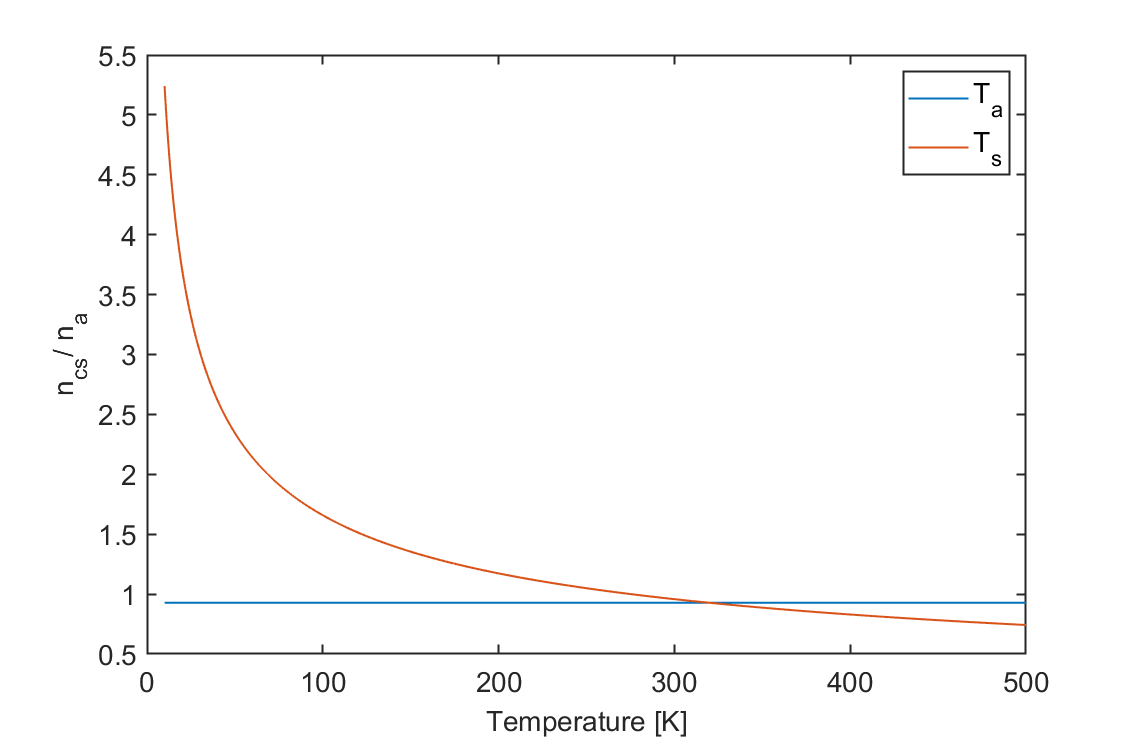
\includegraphics[width= .7\textwidth]{Bilder/Ta_Ts.png}
			\caption{Gain $n_{cs}/n_a$ of the antechamber one time varying the ambient gas temperature $T_a$ and one time varying the antechamber wall temperature $T_s$ according to Eq.\eqref{eq:thDensEnhan}.}
			\label{th:densEnhTaTs}
		\end{figure}
		The next parameter is the radius $r_{aIs}$ of the hole connecting the antechamber with the ionisation region. When the hole gets bigger, also the amount of gas flowing into the ionisation region increases as it can be seen in Fig.\,\ref{th:densEnhraHiraIs}. The radius of the entrance holes $r_{aHi}$ should be small to reach a high gain. This has two reasons: When the entrance holes are big compared to the hole connecting the antechamber with the ionisation region, a big amount of gas flows out through the entrance holes. The size of the entrance holes has also an impact on the opening angle $\omega$. In the first designs of such antechambers, the ionisation and counting of the particles happened in the antechamber itself \cite{Hedin_1964}. Therefore the antechamber needed only one opening. Our instrument has two entrances for particles. One to measure them directly without any interaction with the instrument surface (open-source channel) and a closed-source entrance through the antechamber to amplify the signal. Due to the flyby trajectories of the space craft the antechamber has to entrance holes with angle $\theta_0 = 30\degree$ relative to the x-axis of the instrument.\notes{Rewrite}
		When having only one big entrance hole, the gas gets easily reflected and leaves the antechamber before being counted in the antechamber. Therefore a small opening is favoured over a big opening. From that perspective, the biggest gain is achieved when the radius of the entrance hole is 0 ergo the entrance hole is closed. That's the limitation of Eq.\,\eqref{eq:thDensEnhan} is. It does not take into account that at a certain radius of the opening, the gain should decrease because not enough particles enter the chamber to get amplified.\\
		\begin{figure}[h!] % raHi raIs
			\centering
			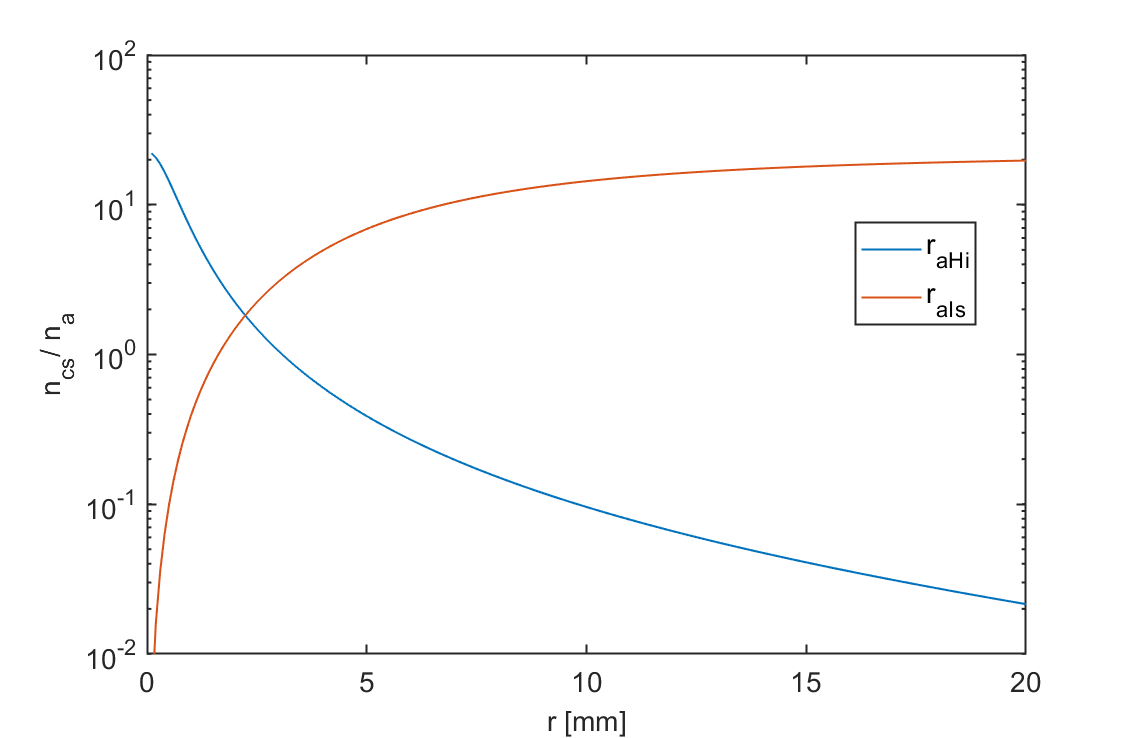
\includegraphics[width= .7\textwidth]{Bilder/raHi_raIs.png}
			\caption{Gain $n_{cs}/n_a$ of the antechamber as a function of the entrance hole radius $r_{aHi}$ and the radius connecting the antechamber with the ionisation region $r_{aIs}$.}
			\label{th:densEnhraHiraIs}
		\end{figure}
		It is very important to take materials with a high particle reflection coefficient $k$ for the coating of the antechamber' s inner surface. The particle reflection coefficient gives the probability of a particle being re-emitted when hitting the surface thus this value has to be close to 1. For our antechamber we used gold because it is electrically conductive preventing the surface from charging in the strong radiation field of Jupiter and it is chemically inert and thus there is a low probability of building chemical bonds with the test gas. Fig.\,\ref{th:densEnhk} shows the amplification of the antechamber in dependence of $k$. When changing $k$ by 1\textperthousand\, this already has a huge impact on the amplification. The impact of $k$ also depends on $\omega$. A small $\omega$ implies a big surface area with which the particles can interact before leaving the antechamber. The more interactions with the antechamber surface are possible, the bigger is the influence of $k$. For our antechamber $\omega$ is about 5.06\,\si{\degree} which is very small and therefore a small change in $k$ has a big impact on the gain.\\
		\begin{figure}[h!] % k
			\centering
			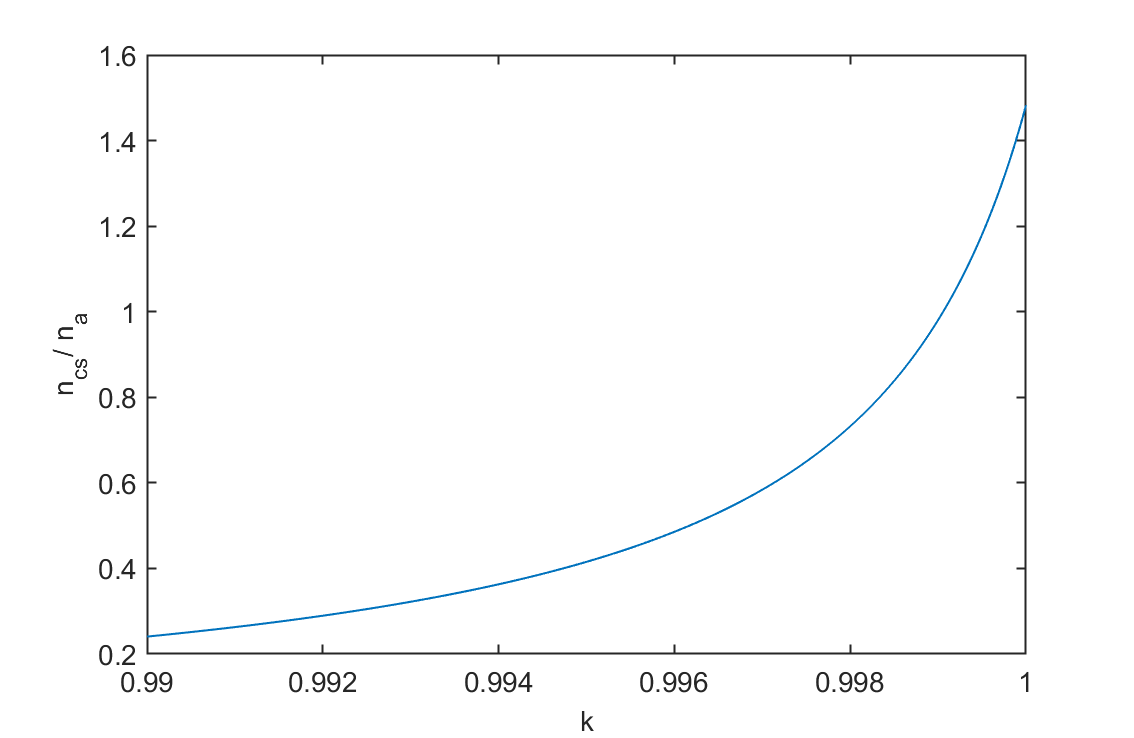
\includegraphics[width= .7\textwidth]{Bilder/k.png}
			\caption{Gain $n_{cs}/n_a$ of the antechamber as a function of the particle reflection coefficient $k$.}
			\label{th:densEnhk}
		\end{figure}
		Fig\ref{th:densEnhm} shows the amplification of the antechamber in dependence of the particles unit mass\,[u]. The figure shows that particles with higher unit mass get amplified more and are therefore easier to detect.\\
		\begin{figure}[h!] % mass
			\centering
			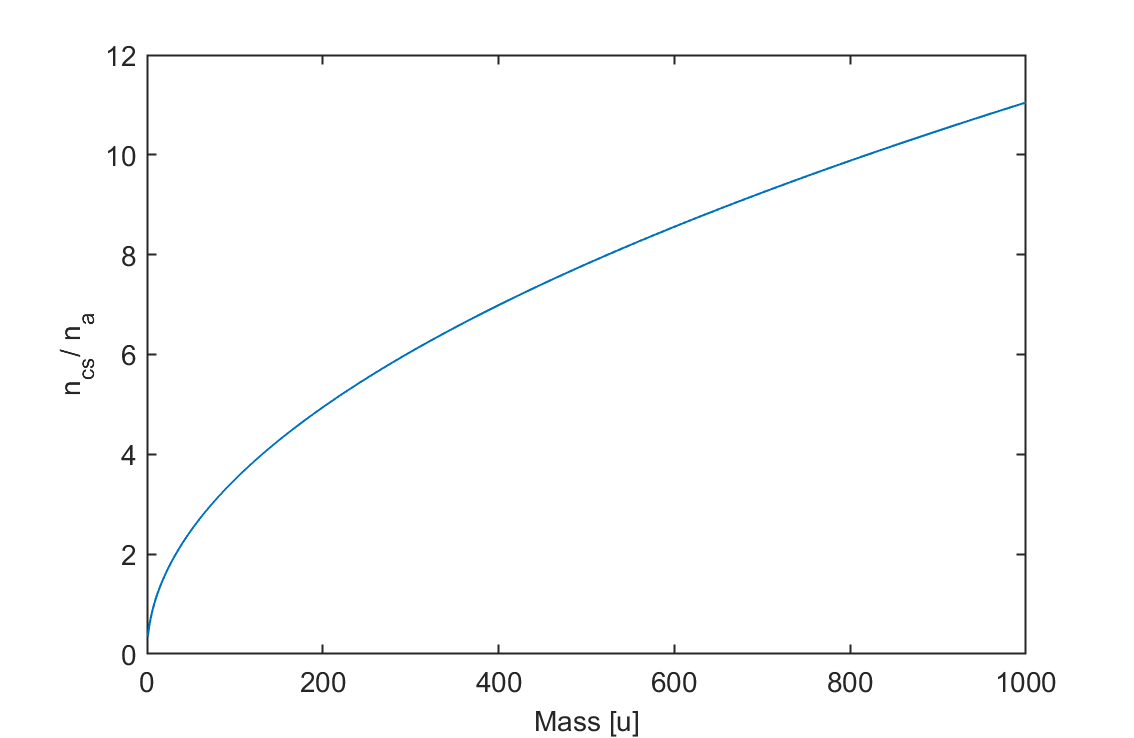
\includegraphics[width= .7\textwidth]{Bilder/m.png}
			\caption{Gain $n_{cs}/n_a$ of the antechamber as a function of the particle mass $m$.}
			\label{th:densEnhm}
		\end{figure}
		Fig.\,\ref{th:densEnhvelo} shows the amplification of the antechamber in dependence of the spacecraft velocity for different species. We expect H\textsubscript{2}O and different radiolysis radiolysis products such as H\textsubscript{2}, O\textsubscript{2} or HO. Absorption lines in the near infrared recorded by the Near Infrared Mapping Spectrometer (NIMS) on board of the Galileo spacecraft indicate CO\textsubscript{2} bond to other solid materials in the soil. Sulphur is part of the plasma. The sulphur compounds are therefore a result of the ion bombardment on the moons surface. Sulphur reacts with water resulting in various different compounds such as sulphur dioxide (SO\textsubscript{2}) or sulphuric acid (H\textsubscript{2}SO\textsubscript{4}) \cite{Collins_2014}. \notes{include Audrey's paper if it gets finished in time.}
		Fig.\,\ref{th:densEnhvelo} shows that with increasing flyby velocity, the particles get more amplified. Species with higher masses are stronger amplified than light particles as it was already shown also in Fig.\,\ref{th:densEnhm}.\\
		\begin{figure}[h!] % velocity
			\centering
			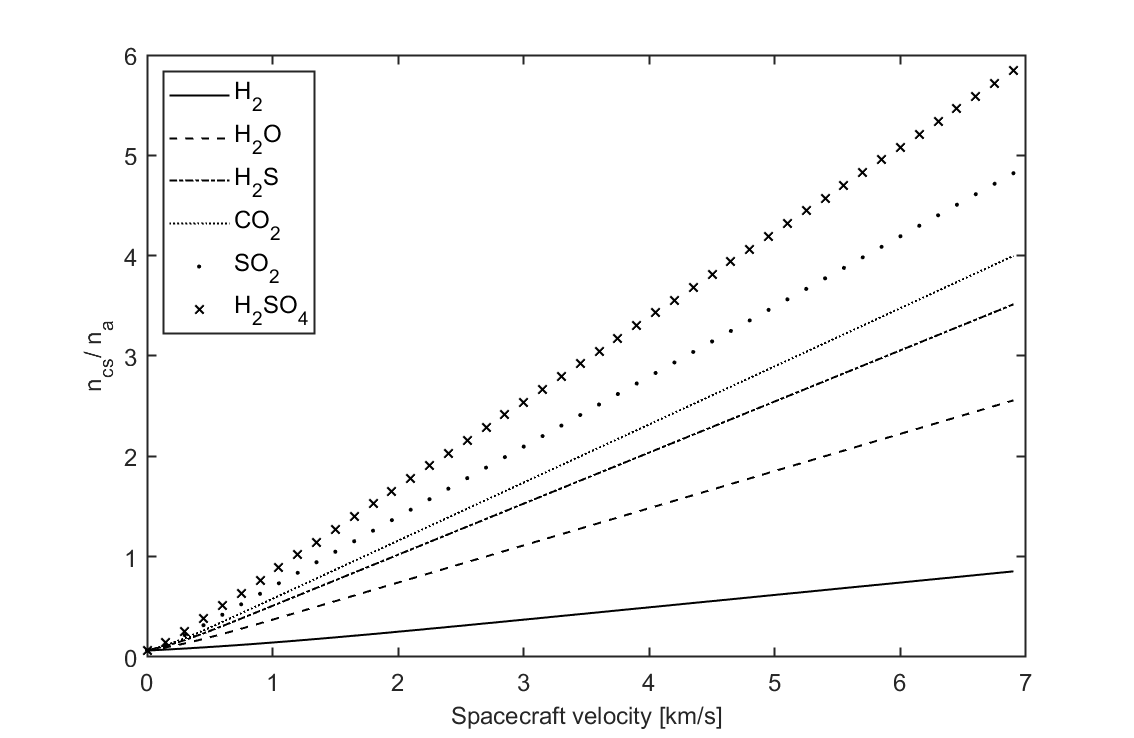
\includegraphics[width= .7\textwidth]{Bilder/velocity.png}
			\caption{Gain $n_{cs}/n_a$ of the antechamber as a function of the spacecraft velocity $v_{sc}$ for different species expected in the moons atmospheres.}
			\label{th:densEnhvelo}
		\end{figure}
		Fig.\,\ref{th:densEnhChiTheta} shows the amplification in dependence of different particle influx angles $\chi$. $\chi$ is measured in the x-/y- plane (Fig.\,\ref{fig:thAntIs}). The function was evaluated for different positions of the entrance holes. The minimal angle the two entrance hole can be apart from each other without overlapping is 3.6\si{\degree}. The holes of the PFM are at $\theta_0 = \pm30\,\si{\degree}$. With that configuration the biggest signal intensity is measured with a spacecraft ramp direction of 0\si{\degree}. When the two holes are at $\pm$60\si{\degree} it results in a plateau between $\pm$60\,\si{\degree} and also a wider angular range at which NIM is sensitive. This is an interesting feature under certain circumstance. For our purpose it is unnecessary because the spacecraft blocs the field of view (FoV) for angles bigger than 100\degree (see also Chap.\,\ref{subsubsec:Calfly}).
		\begin{figure}[h!] % chi theat
			\centering
			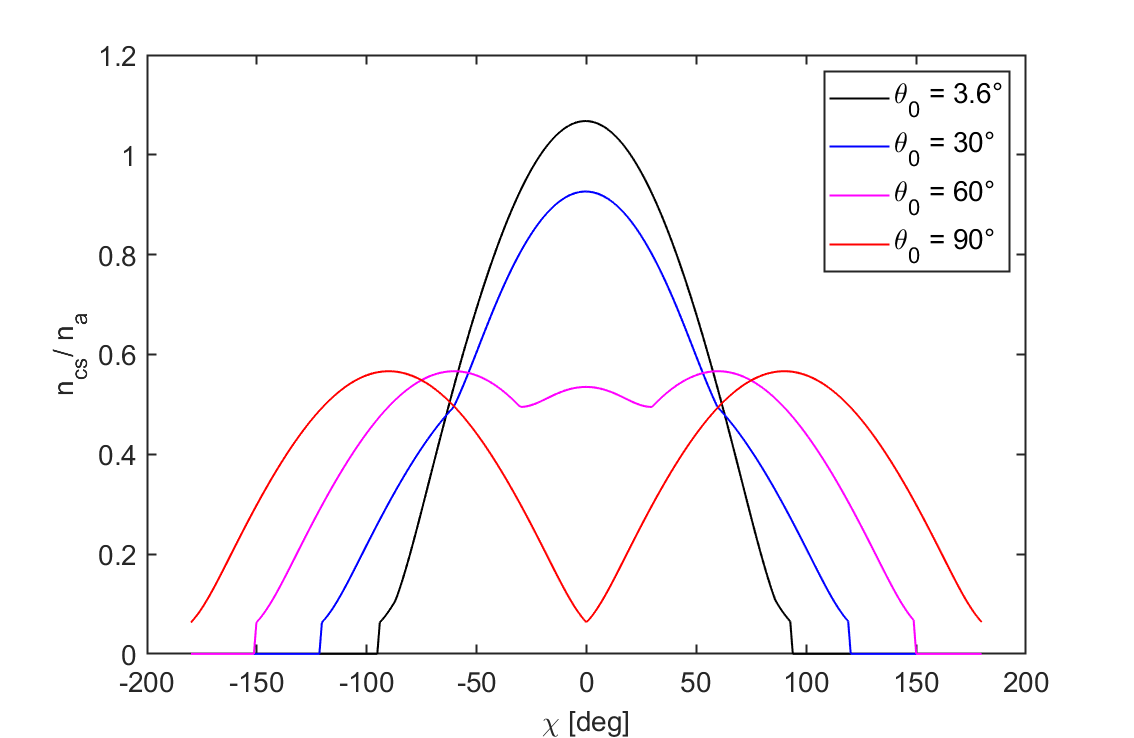
\includegraphics[width= .8\textwidth]{Bilder/Chi_theta0.png}
			\caption{Gain $n_{cs}/n_a$ of the antechamber as a function of the gas influx direction $\chi$ for different positions of the two entrance holes $\theta_0$. $\theta_0=30\degree$ is the position of the holes in flight configuration.}
			\label{th:densEnhChiTheta}
		\end{figure}
		
%-------------------------------------------------------------------------------------------		
		\subsubsection{Callisto Flyby}\label{subsubsec:Calfly}
	
		\begin{figure}[h!]
			\centering
			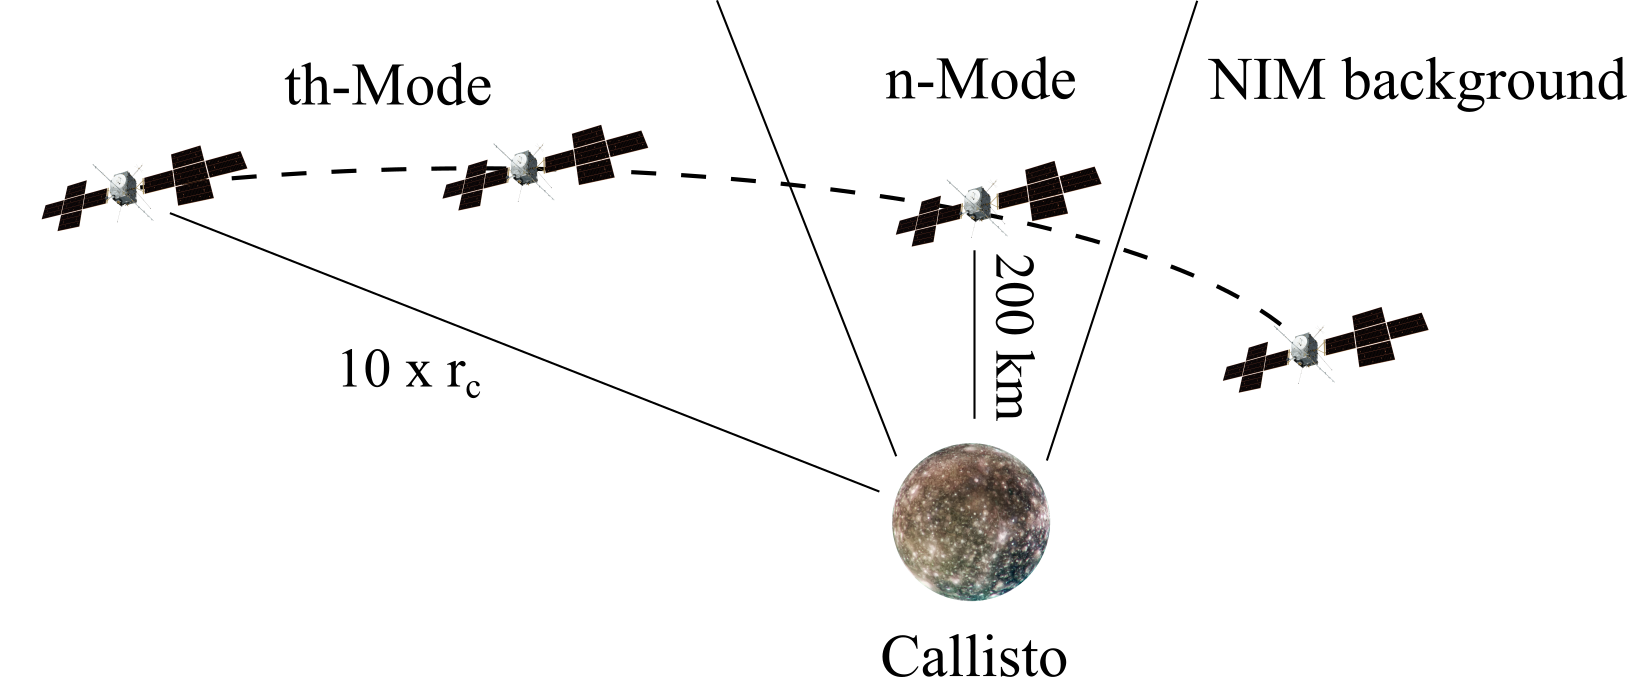
\includegraphics[width=.8\textwidth]{Bilder/Callisto_flyby_schematic.png}
			\caption{Schematics of one of the flybys at Jupiter's moon Callisto.}
			\label{fig:CalflybySchem}
		\end{figure}
				
		\begin{figure}[h!]
			\centering
			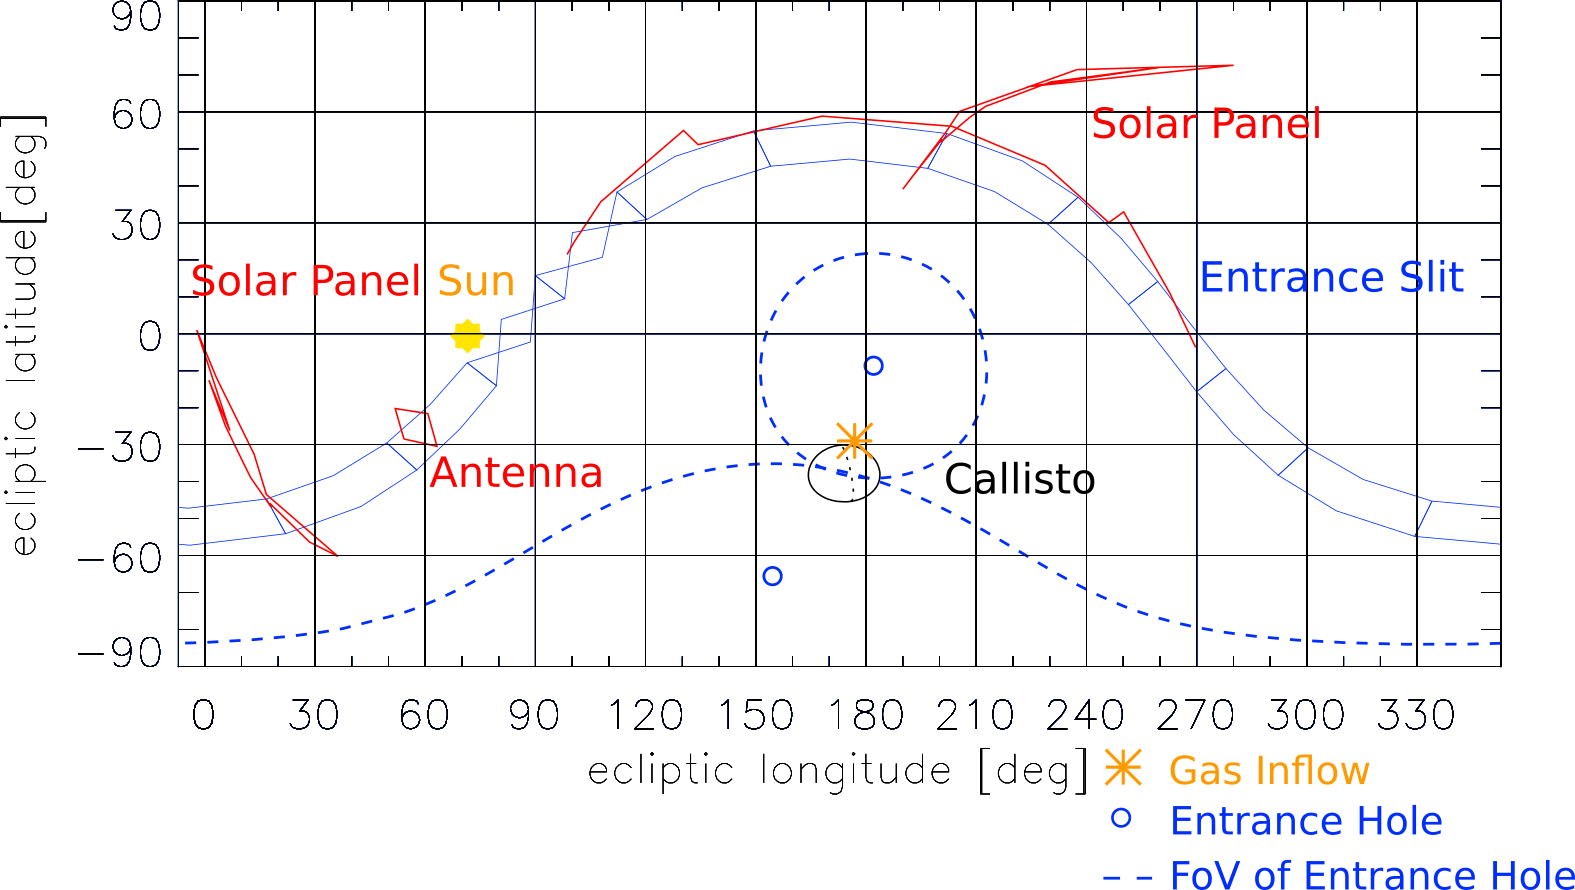
\includegraphics[width = .7\textwidth]{Bilder/NIM_pointing_2031JAN15185200.png}
			\caption{Fourth Callisto flyby of trajectory 141a \cite{SOC_Crema3p2} 1\,h before closest approach 15'600\,km away from Callisto.}
			\label{fig:FlybyCal1852}
		\end{figure}
		\begin{figure}[h!]
			\centering
			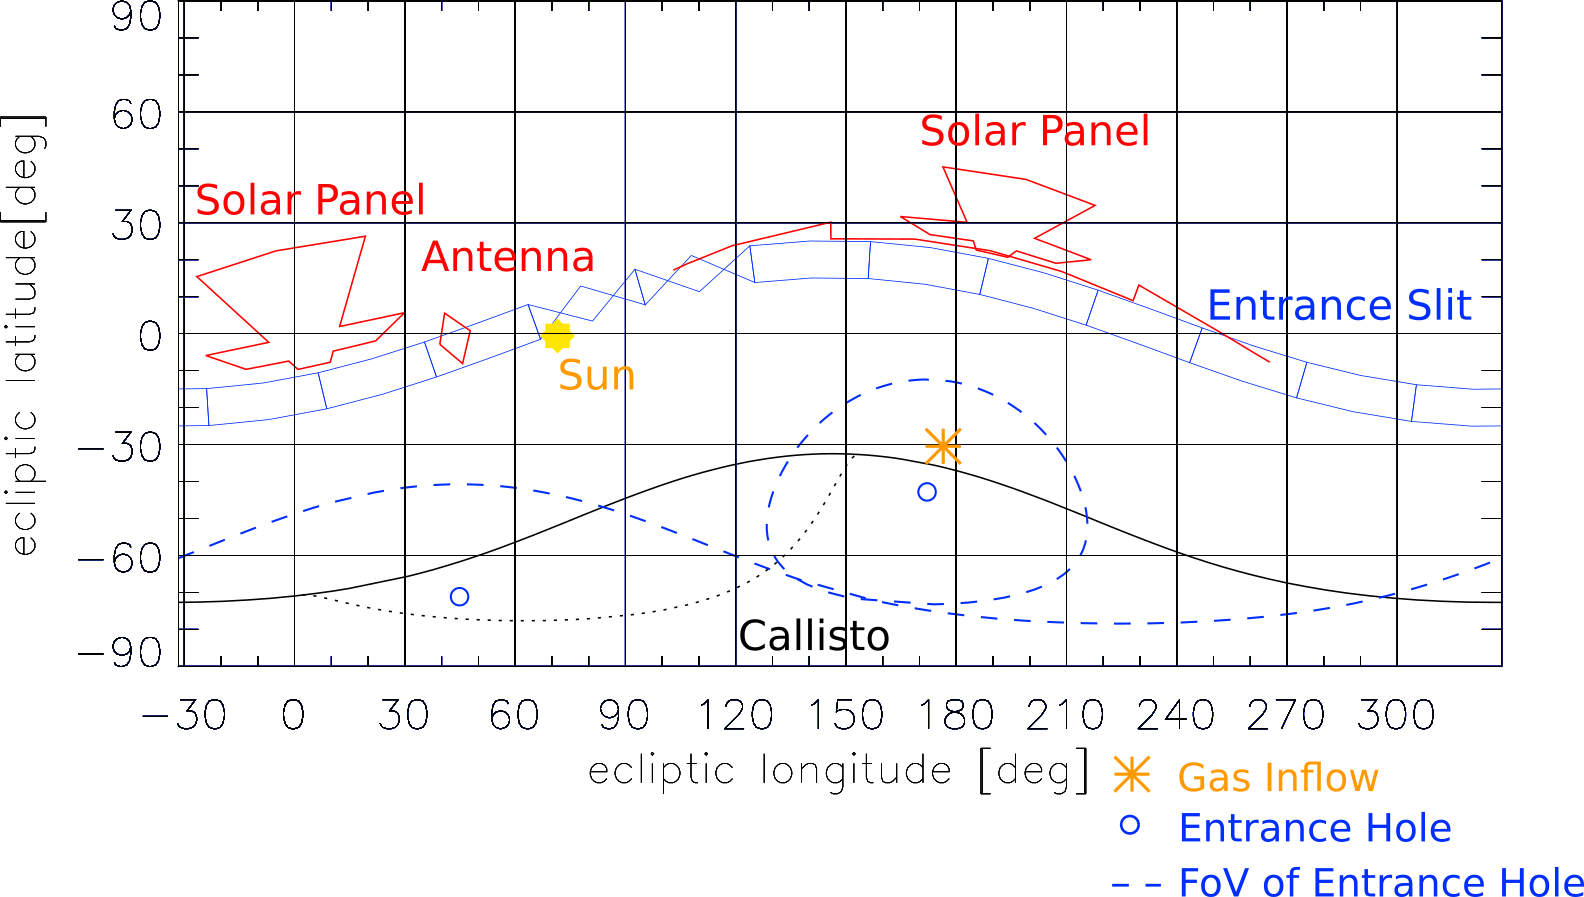
\includegraphics[width = .7\textwidth]{Bilder/NIM_pointing_2031JAN15194200.png}
			\caption{Fourth Callisto flyby of trajectory 141a \cite{SOC_Crema3p2} 10\,min before closest approach 1'560\,km away from Callisto.}
			\label{fig:FlybyCal1942}
		\end{figure}
		\begin{figure}[h!]
			\centering
			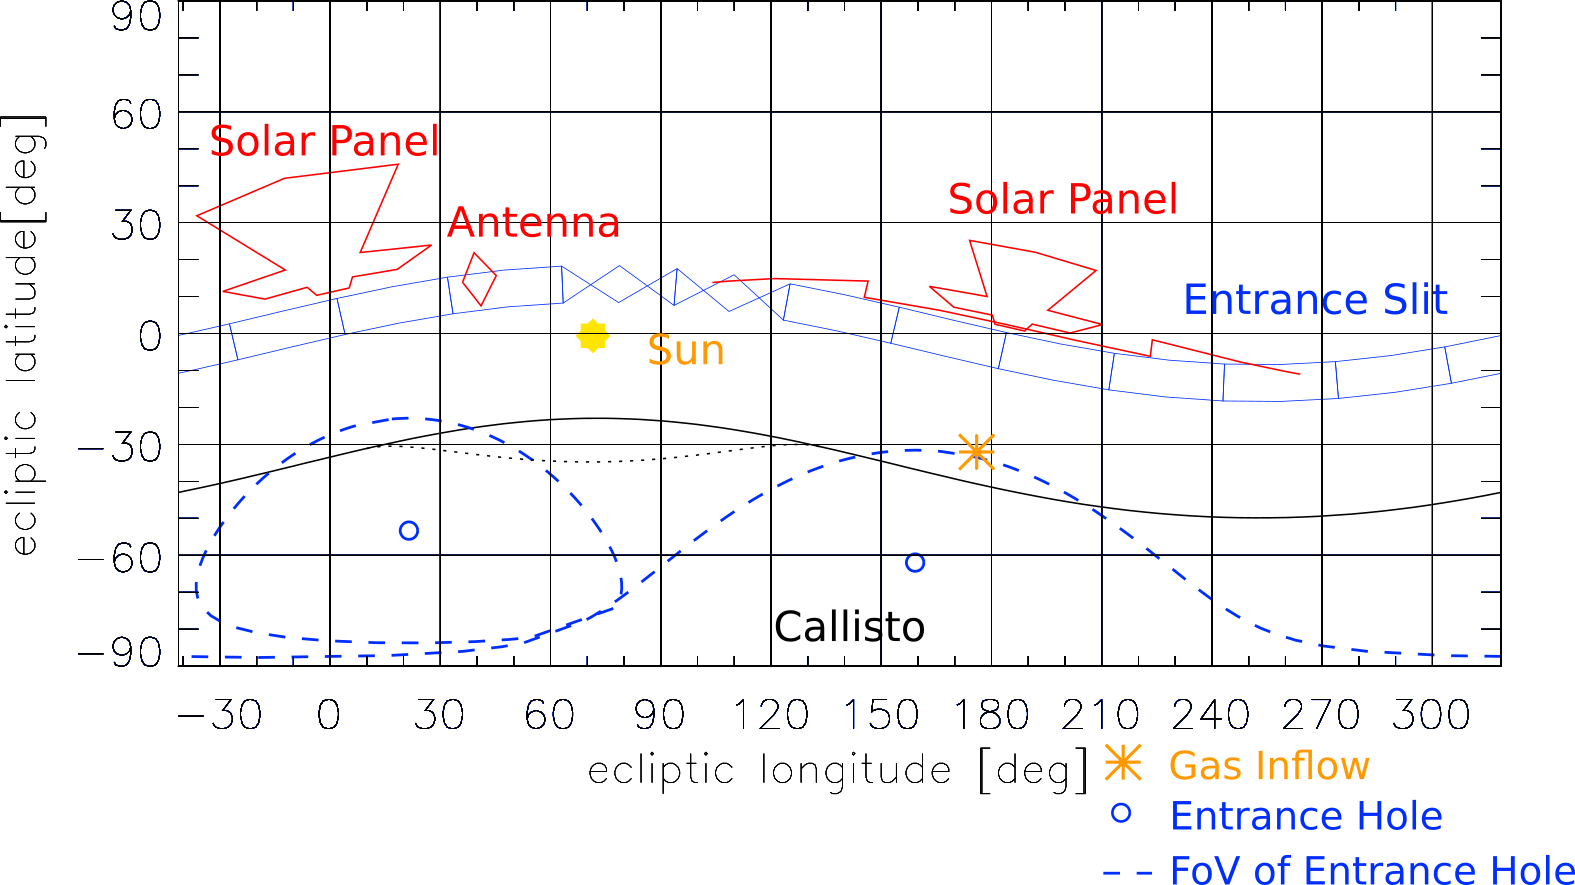
\includegraphics[width = .7\textwidth]{Bilder/NIM_pointing_2031JAN15194700.png}
			\caption{Fourth Callisto flyby of trajectory 141a \cite{SOC_Crema3p2} 5\,min before closest approach 580\,km away from Callisto.}
			\label{fig:FlybyCal1947}
		\end{figure}
		\begin{figure}[h!]
			\centering
			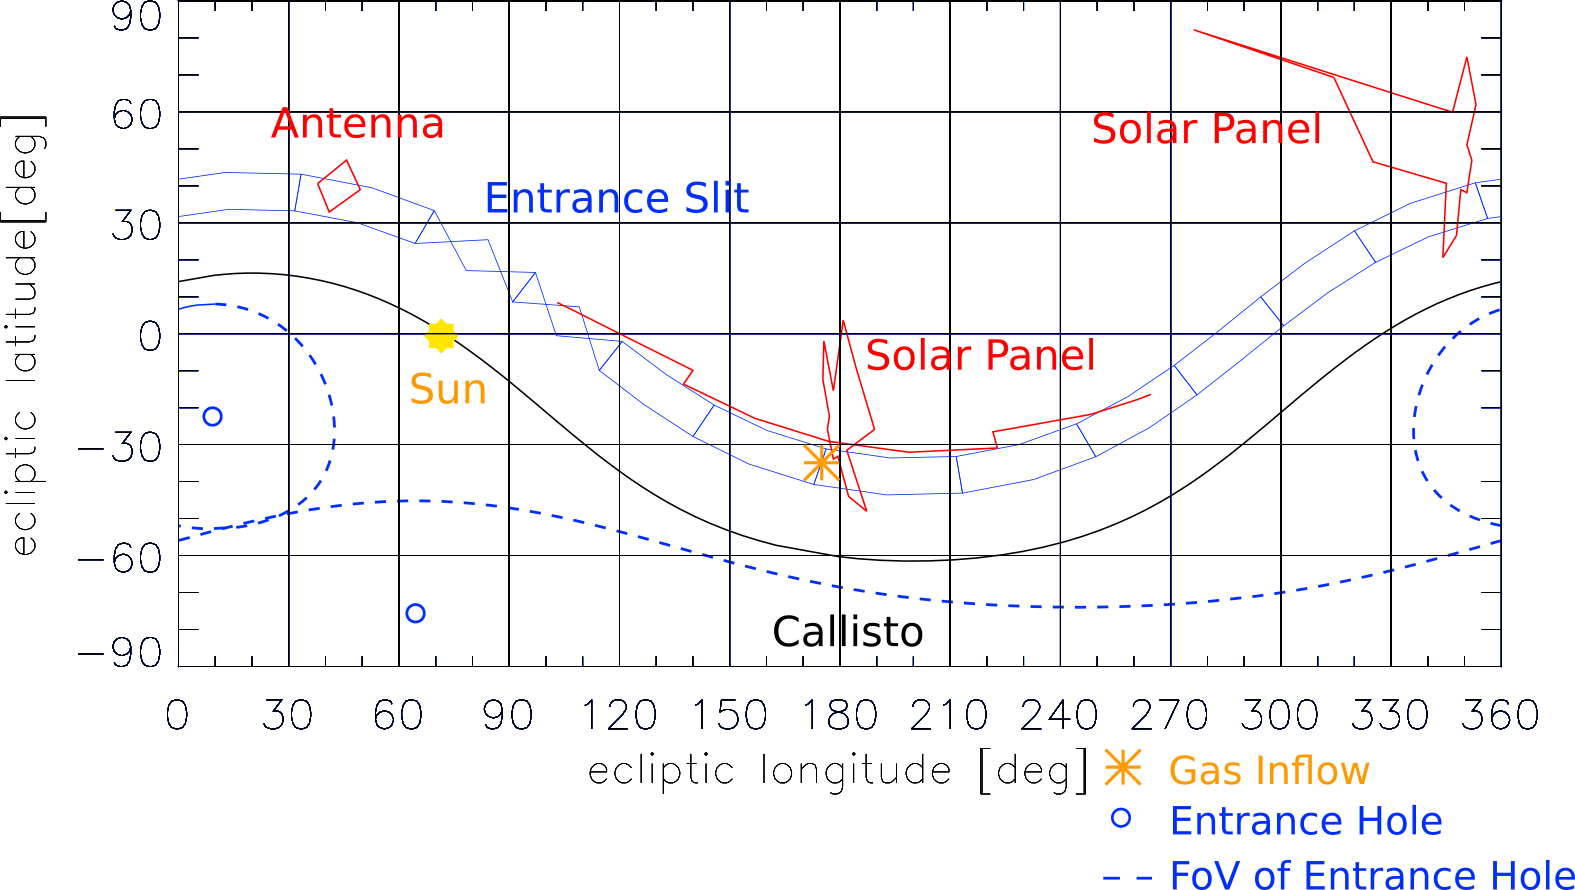
\includegraphics[width = .7\textwidth]{Bilder/NIM_pointing_2031JAN15195200_tilt.png}
			\caption{Fourth Callisto flyby of trajectory 141a \cite{SOC_Crema3p2} closest approach 200\,km away from Callisto with the solar panels oriented toward the sun to maximizes power generation of the spacecraft.}
			\label{fig:FlybyCal1952sol}
		\end{figure}
		\begin{figure}[h!]
			\centering
			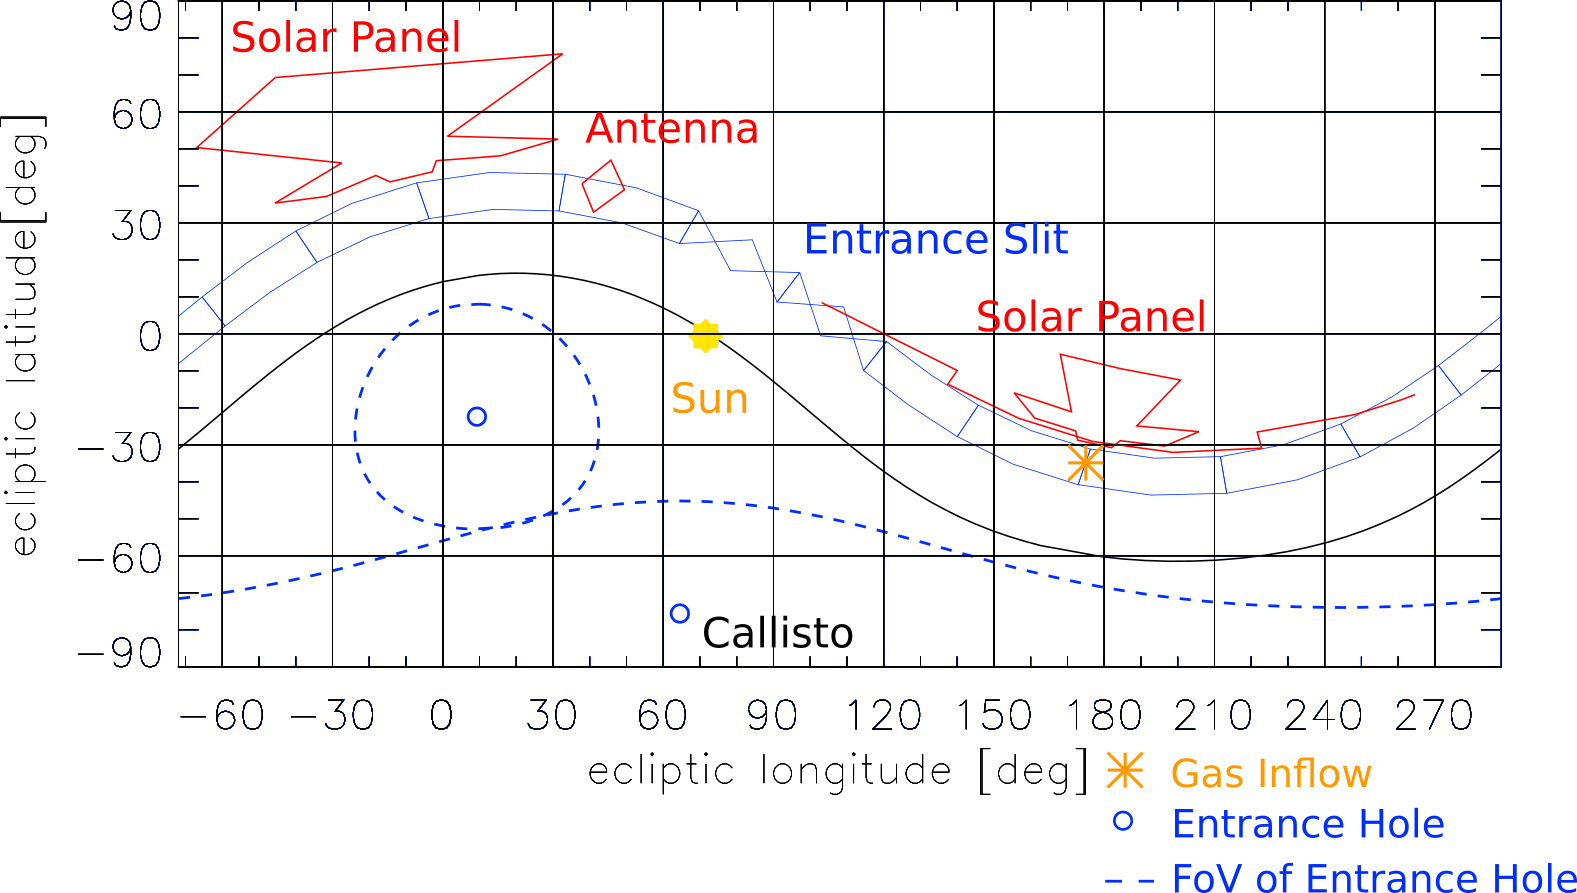
\includegraphics[width = .7\textwidth]{Bilder/NIM_pointing_2031JAN15195200.png}
			\caption{Fourth Callisto flyby of trajectory 141a \cite{SOC_Crema3p2} closest approach 200\,km away from Callisto.}
			\label{fig:FlybyCal1952}
		\end{figure}
		\begin{figure}[h!]
			\centering
			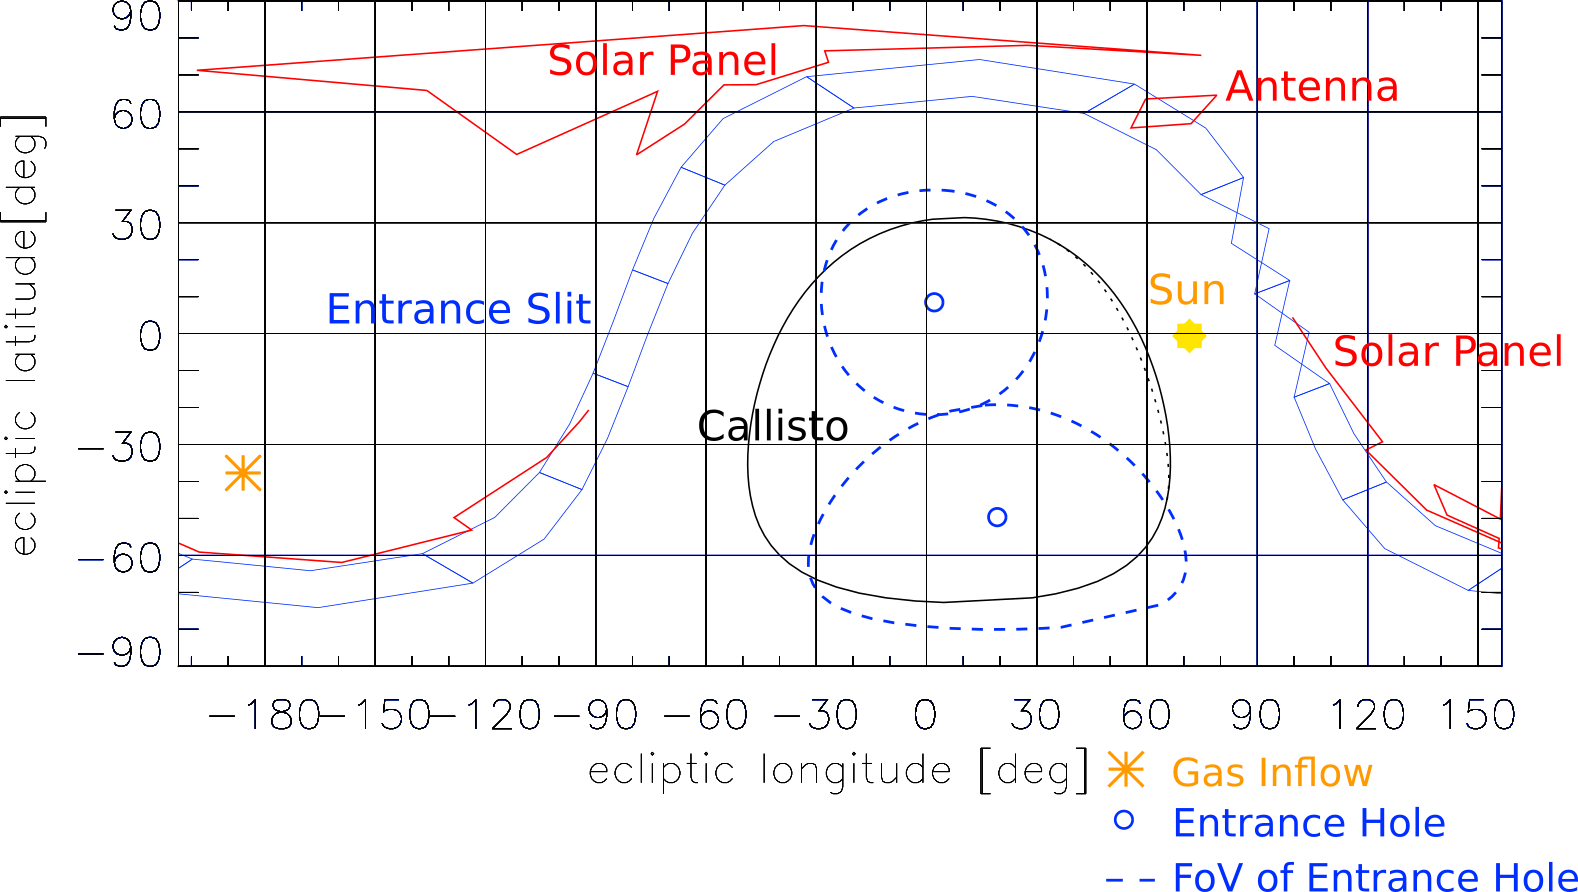
\includegraphics[width = .7\textwidth]{Bilder/NIM_pointing_2031JAN15195700.png}
			\caption{Fourth Callisto flyby of trajectory 141a \cite{SOC_Crema3p2} 5\,min after closest approach 640\,km away from Callisto.}
			\label{fig:FlybyCal1957}
		\end{figure}
		Fig.\,\ref{fig:FlybyCal1852}\,- Fig.\,\ref{fig:FlybyCal1957} show the changing FoV of the NIM instrument at different times during the fourth Callisto flyby of trajectory 141a \cite{SOC_Crema3p2}. The reference coordinate system for these graphics is the ecliptic coordinate system. During the flyby, the spacecraft changes its orientation in reference to that coordinate system leading to a distortion of the different objects in the figures. The entrance holes of the antechamber are blue circles, the FoVs of the entrance holes are marked as dashed blue lines, the entrance slit is the blue band with the sinusoidal shape. The solar panels and the antenna which bloc part of the FoV of NIM are marked in red. The gas inflow direction is marked as an orang star. Fig.\,\ref{fig:FlybyCal1852} shows the FoV 1\,h before closest approach 15'600\,km above Callisto's surface. The gas inflow direction is in between the two entrance holes. The black doted line on the moons surface marks the day/night separation line. As the spacecraft moves closer to the moon, the gas inflow direction moves towards the entrance slit. 5\,min before closest approach, NIM changes from thermal to neutral mode (Fig.\,\ref{fig:FlybyCal1947}) to be ready for the neutral mode measurements. At this time, the gas inflow direction is still in the FoV of the antechamber. The time window for measuring with the neutral gas mode is very narrow. Already 5\,min after closest approach, the gas inflow direction is below the FoV of the neutral gas channel (Fig.\,\ref{fig:FlybyCal1957}). Therefore, the time to switch from thermal to neutral mode has to be very short to minimize the number of lost measurements. These measurements are very crucial because the closer the spacecraft gets to the moon's surface, the higher is the exospheric pressure and therefore the signal intensity.\\
		The spacecraft structure blocs angles higher than 100\si{\degree}. The gas striking the spacecraft sputters particles from the spacecraft's surface. NIM is not able to determine if these particles are part of the moons exosphere of if they originate from the spacecraft. When the gas inflow direction reaches angles higher than 100\si{\degree} NIM starts measuring background. The solar panels are adjusted perpendicular to the sun to maximize power generation. 10\,min before closest approach, the solar panels are tilted to leave open the FoV of NIM to measure with the neutral gas mode. In case the solar panels would stay perpendicular to the sun, the gas would graze the surface of the solar panel as it is shown in Fig.\,\ref{fig:FlybyCal1952sol}. Fig.\,\ref{fig:FlybyCal1952} shows the same scenario but with the solar panels tilted to leave open NIM's FoV of the neutral gas channel.\\
		Fig.\,\ref{fig:densEnhChiFlyby} shows the gain of the antechamber with the total FoV of the two entrance holes marked as red area $\pm$30\degree around the position of the two entrance holes. The orange stars mark the gas inflow direction for the various scenarios mentioned before.
		\begin{figure}[h!]
			\centering
			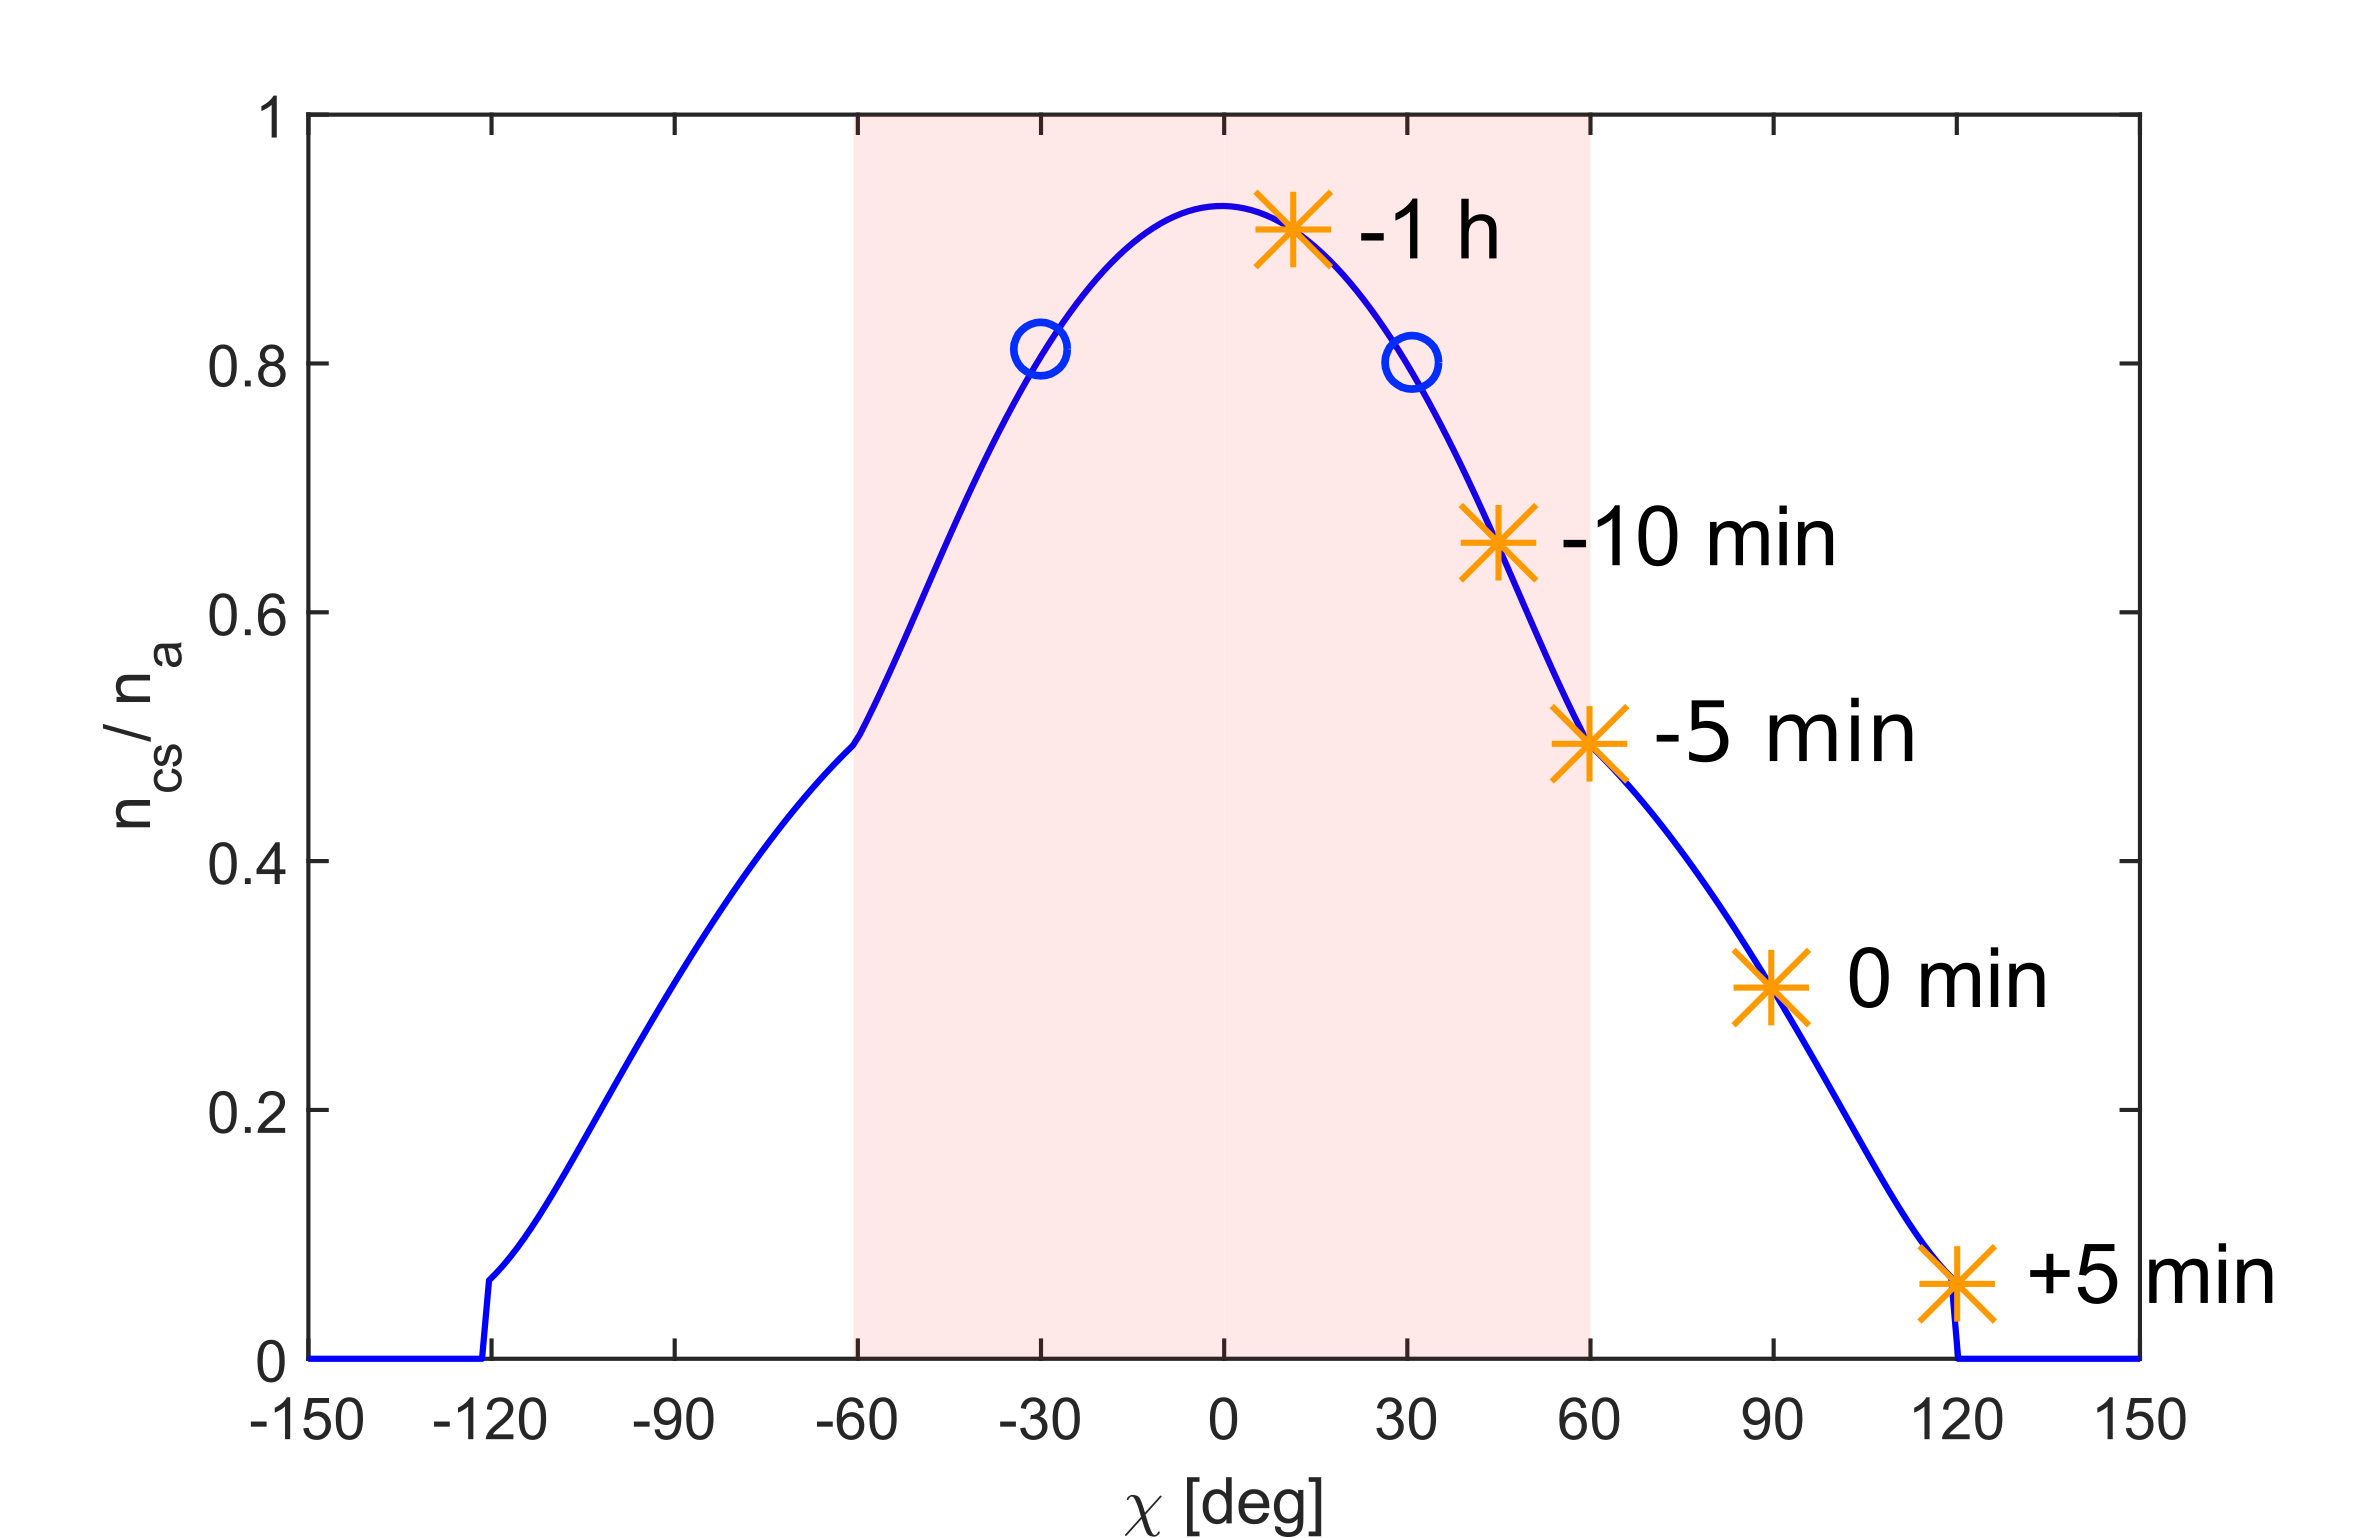
\includegraphics[width=.8\textwidth]{Bilder/Chi_theta0_flyby.png}
			\caption{Gain $n_{cs}/n_a$ of the antechamber in dependence of the gas influx direction $\chi$. The blue circles mark the entrance hole positions and the red area marks the FoV of the entrance holes. The stars mark the gas influx direction from 1\,h before until 5\,min after closest approach of trajectory 141a \cite{SOC_Crema3p2}.}
			\label{fig:densEnhChiFlyby}
		\end{figure}
		The main gas inflow direction varies for the different flybys. One time the gas comes from positive and one time from negative $\chi$ direction. Therefore, it was decided to make two entrance holes to allow measurements with angles different to the main direction to enlarge the FoV of the antechamber. The holes should also not be too close at the entrance because structures of the spacecraft bloc angles bigger than 100\degree and an amplification of such big angles would be useless.
		
		
%----------------------------------------------------------------------------------		
		\subsubsection{Shutter Performance} \label{subsubsec:motorflow}
		NIM has a shutter to close the entrance to the antechamber. This shutter is mounted between the ion source and the antechamber (Fig.\,\ref{fig:shutterMotor} left). When the shutter is open, the gas flows right through the hole into the ion source. When the shutter is closed, the hole moves to the side as it is indicated in Fig.\,\ref{fig:shutterMotor} right. Because the shutter does not close the gag perfectly, still a small amount of gas flows around the shutter into the ionisation region. In the following section, the geometry factor $G_{close}$ of the antechamber is determine when the shutter is closed.\\
		\begin{figure}[h!]
			\begin{subfigure}{0.5\textwidth}
				\centering
				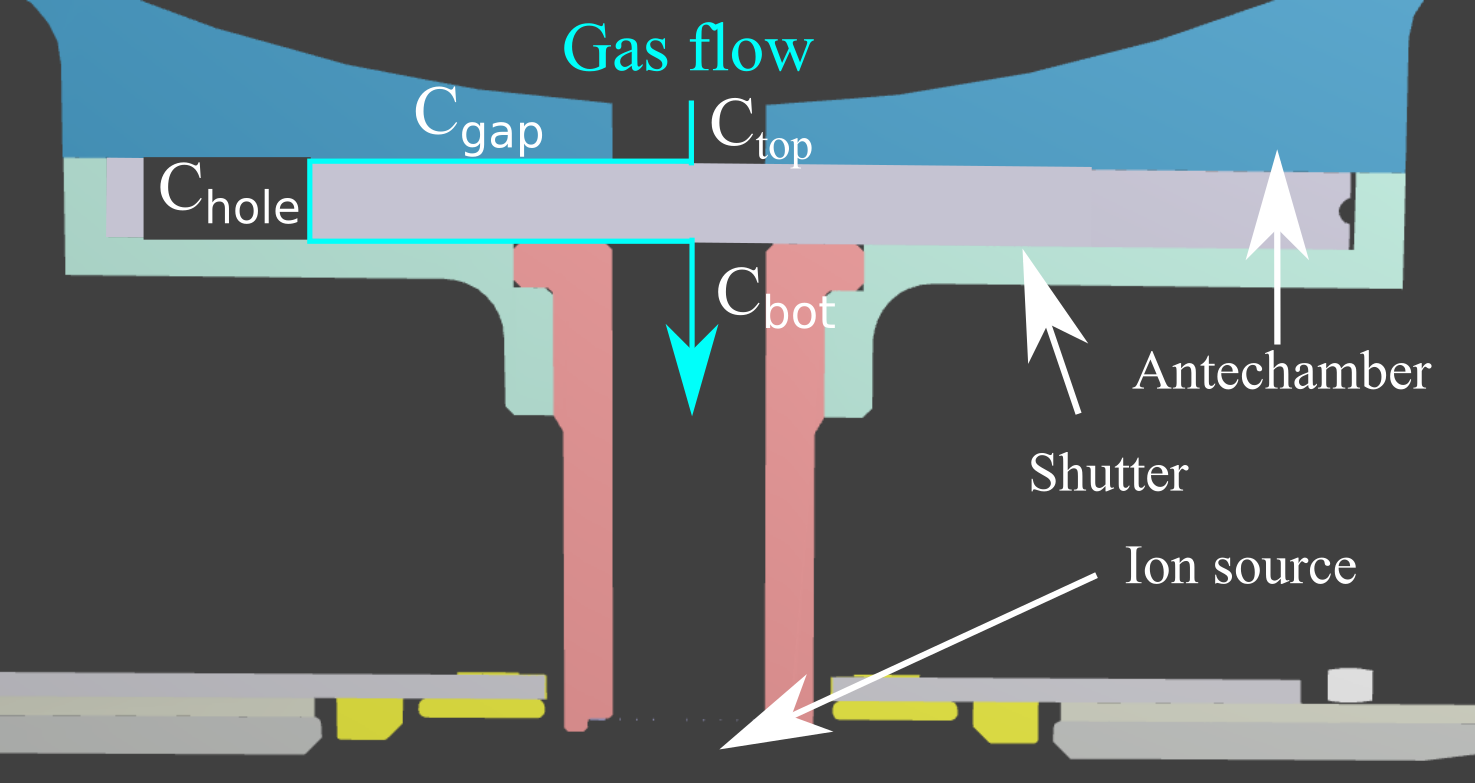
\includegraphics[width=\textwidth]{Bilder/Shutter_sideview.png}
			\end{subfigure}
			\begin{subfigure}{0.5\textwidth}
				\centering
				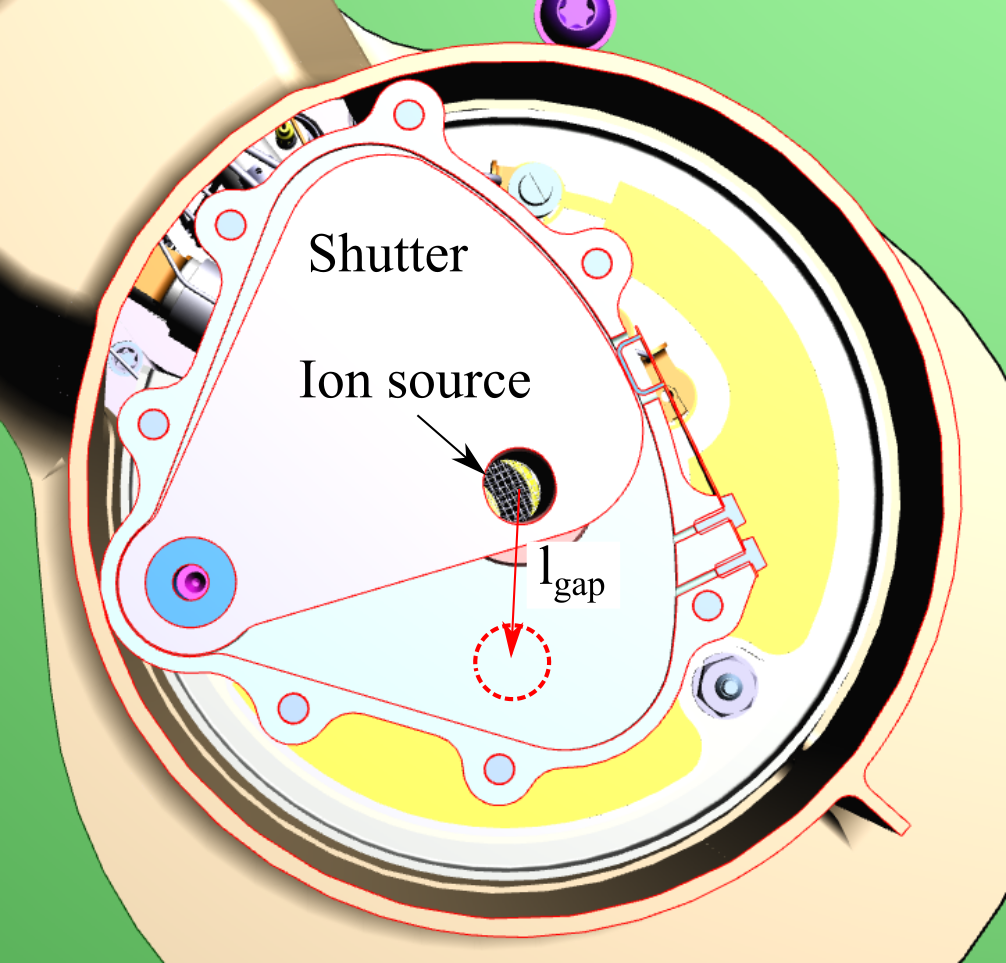
\includegraphics[width=.8\textwidth]{Bilder/Shutter_topview.png}
			\end{subfigure}
		\caption{Shutter Motor. Left: side view with shutter closed. Right: Top view with open shutter. When the shutter is closing the central hole moves to the red position.}
		\label{fig:shutterMotor}
		\end{figure}
		The molecular flow conductance is:
		\begin{equation}
			C = \frac{A\cdot\bar{v}\cdot a}{4}
		\end{equation}
		With $A$ the cross-section of the tube, $\bar{v}$ the average velocity of the thermalized gas flowing through the opening and $a$ the transmission probability depending on the length-to-diameter ratio of the tube. When the shutter is closed, the conductance of the tube $C_{tot}$ is divided into four terms: The conductance of the upper part of the tube $C_{top}$, the conductance of the gap between the shutter and pocket $C_{gap}$, the conductance of the hole in the shutter $C_{hole}$ and the conductance of the lower part of the tube connecting the antechamber with the ionization region $C_{bot}$ (Fig.\ref{fig:shutterMotor} left):
		\begin{align}
			C_{top}  &= \frac{r_{aIs}^2\cdot\pi\cdot\bar{v}\cdot a_{top}}{4}\\
			C_{gap}  &= \frac{2\cdot r_{aIs}\cdot \pi \cdot h_{gap}\cdot\bar{v}\cdot a_{gap}}{4}\\
			C_{hole} &= \frac{r_{aIs}^2\cdot\pi\cdot\bar{v}\cdot a_{hole}}{4}\\
			C_{bot}  &= \frac{r_{aIs}^2\cdot\pi\cdot\bar{v}\cdot a_{bot}}{4}
		\end{align}
		\begin{table}[h!]
			\begin{center}
				\begin{tabular}{l r| l r }
					$a_{top}$	& 0.73 	& $h_{top}$		& 1.5\,mm	\\
					$a_{gap}$	& 0.07 	& $h_{gap}$		& 0.01\,mm \\
					$a_{hole}$ 	& 0.67 	& $h_{hole}$ 	& 2\,mm\\
					$a_{bot}$ 	& 0.28 	& $h_{bot}$ 	& 12\,mm\\
					$r_{aIs}$ 	& 2\,mm & $l_{gap}$ 	& 7\,mm\\
				\end{tabular}
			\end{center}
			\caption{Nominal transmission probabilities $a_i$, tube heights $h_i$, tube radius $r_{aIs}$ and minimal gap length $l_{gap}$ when the shutter between the antechamber and the ion-source is closed.}
			\label{tab:thMolFloConMotClosPara}
		\end{table}	
		With $a_{i}$ the transmission probabilities of the different sections (Eq.\,\eqref{eq:MolFloConFitFunc}), $h_i$ the height of the different sections, $r_{aIs}$ the radius of the antechamber hole and $l_{gap}$ the minimal distance between the hole in the shutter and the tube connecting the antechamber with the ion-source. The nominal values for these parameters are listed in Table\,\ref{tab:thMolFloConMotClosPara}. The average velocity $\bar{v}$ will cancel out later in the derivation of the geometry factor. The conductance of the tube $C_{tot}$ is:
		\begin{equation}
			\frac{1}{C_{tot}} = \frac{1}{C_{top}} + \frac{2}{C_{gap}} + \frac{1}{C_{hole}} + \frac{1}{C_{bot}}
		\end{equation}
		The conductance of one of the entrance holes of the antechamber is:
		\begin{equation}
			C_{aHi} = \frac{r_{aHi}^2\cdot\pi\cdot\bar{v}}{4}
		\end{equation}
		The geometry factor of the tube when the shutter is closed $G_{close}$ is:
		\begin{equation}
			G_{close} = \frac{C_{tot}}{C_{tot} + 2\cdot C_{aHi}}
		\end{equation}
		\begin{figure}[h]
			\centering
			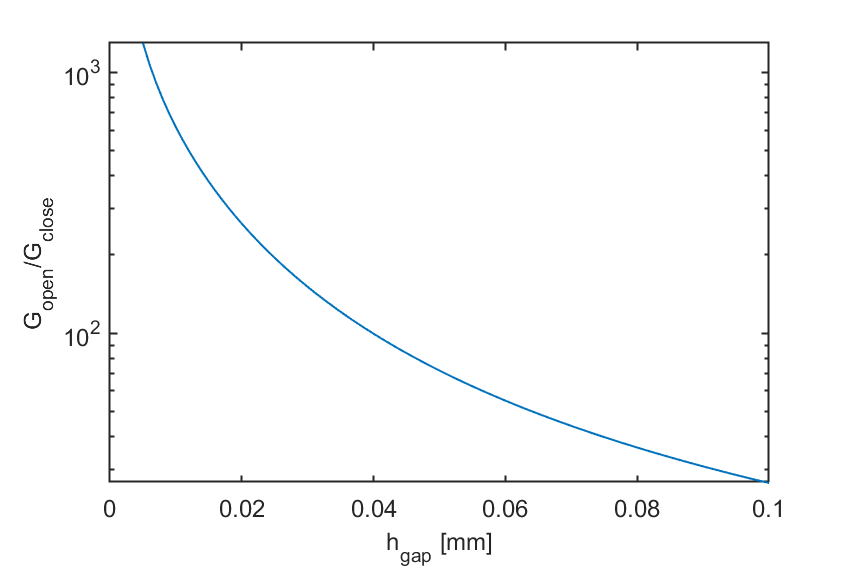
\includegraphics[width=.8\textwidth]{Bilder/ShutGapSizeSigDamp.png}
			\caption{Damping factor $G_{open}/G_{close}$ of the shutter as a function of the gap size $h_{gap}$ of the gap between the shutter and antechamber.}
			\label{fig:ShutGapSizeSigDamp}
		\end{figure}
		The gap between the shutter and the antechamber has to be very thin to seal the hole when the shutter is closed. Fig.\,\ref{fig:ShutGapSizeSigDamp} shows the damping factor $G_{open}/G_{close}$ as a function of the gap size $h_{gap}$. With increasing gap size, the damping factor reduces significantly. The requirement was to damp the signal by a factor 1000 when the shutter is closed. With the nominal gap size of 0.01\,mm, the shutter damps the signal by a factor 600. When the gap size is about 0.1\,mm the damping factor is only about 25. This may can happen when the shutter is not properly fabricated and the tolerances are therefore bigger than originally designed.\\
		When measuring with the open source channel, a small amount of gas will enter the ion-source through the antechamber. The open source slit is in the y-/z-plane and therefore $\chi$ is 90\si{\degree} (Fig.\ref{fig:thAntIs}). When the shutter is closed, about 0.05\% of the signal originates from the antechamber.
		
		%In this approximation the assumption was that the gas will take the shortest distance between the antechamber and the ion-source. In reality it will flow around the shutter and the signal will be damped even more because with increasing distance the gas has to flow, it get damped more.
		
		\subsubsection{Pulser}
		% Draw a second schema of the pulser to compare the rise time/ energy distributions. Or just make a zoom on the falling edge of the pulse and explain it with the energy why a certain configuration is favourable.
		
		% Analysis of the timeings.
		% -> discussion about the time focussing of the reflectron and for how much it can compensate.
		
		
		% Pulse shape is discussed with the flight pulse as an example. May that comes in the experimental part thus it discusses hardware...
		
		\begin{figure}[h]
			\centering
			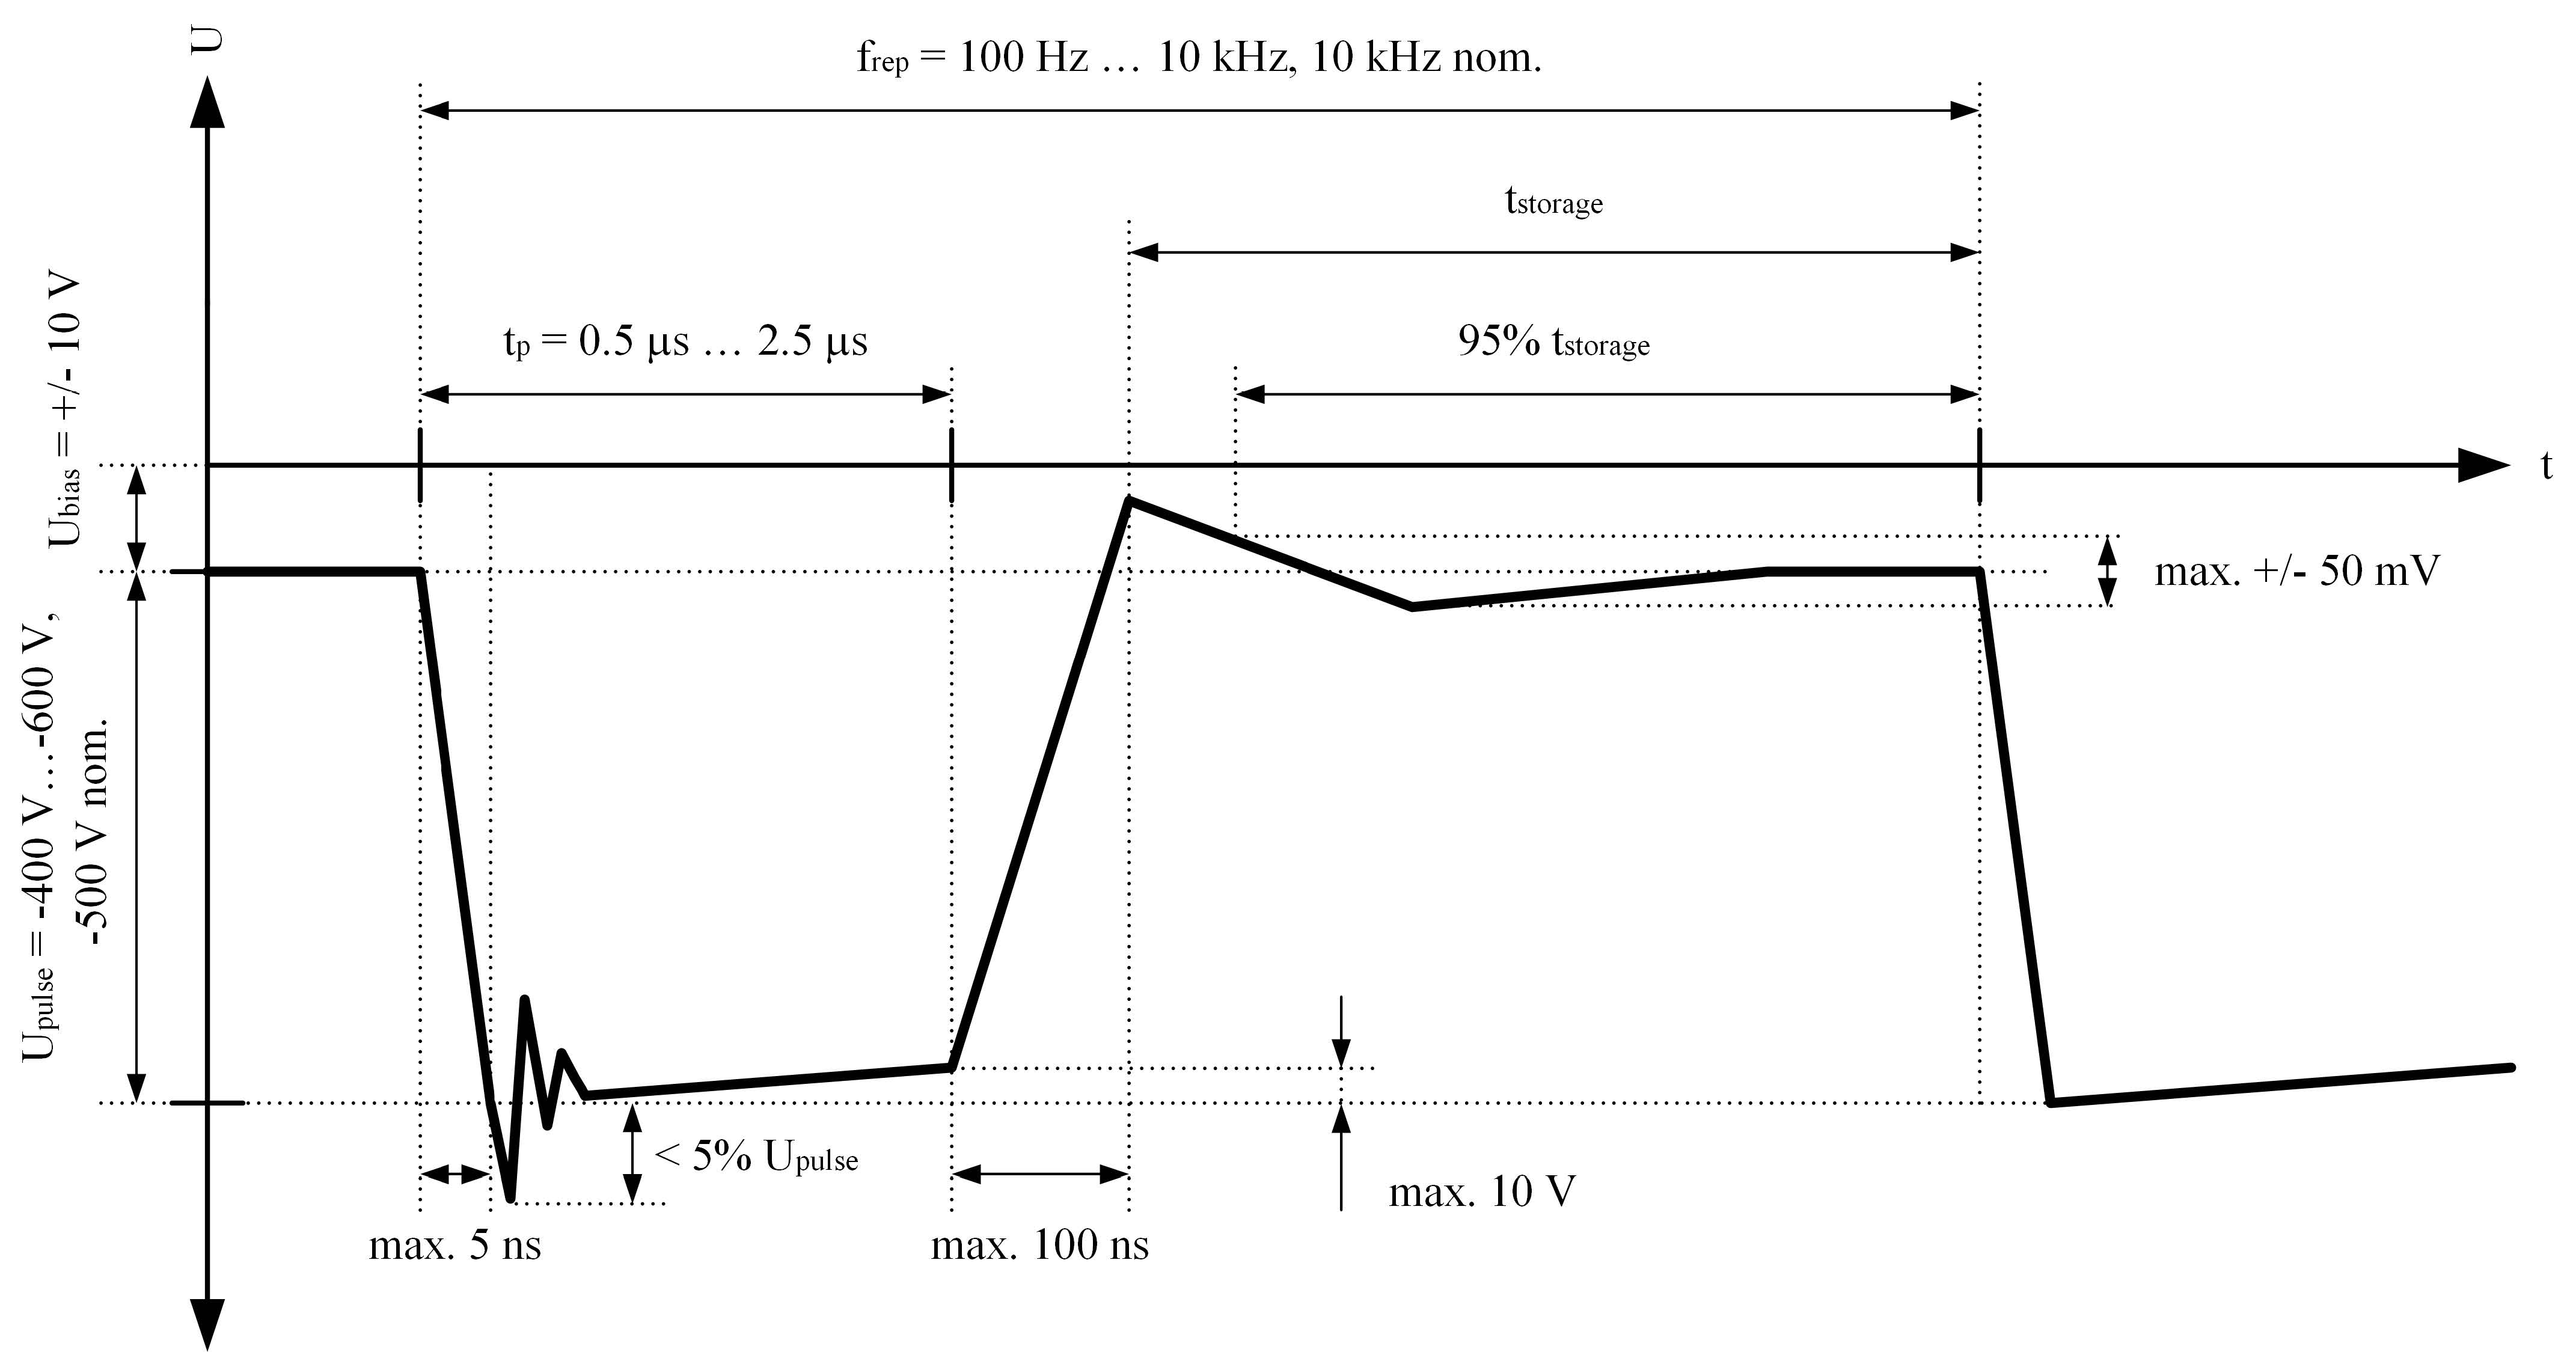
\includegraphics[width=\textwidth]{Bilder/Pulser_theretical_shape.jpg}
			\caption{Specifications for the pulse shape generated by a realistic pulser \cite{Diss_Meyer}.}
			\label{fig:PulserTheoCurve}
		\end{figure}
		The high voltage pulser is used to accelerate the generated ions in the ionisation region to a certain energy. During the time when no high voltage pulse is applied, the potential has to be stable at the bias voltage to allow ion storage as previously discussed in chapter\,\ref{chap:IonStor}.\\ Fig.\,\ref{fig:PulserTheoCurve} shows a schema of a realistic high voltage pulse and Table\,\ref{tab:FlightPulserPerf} shows the characteristics of the flight pulser compared to the requirements. The fall time is the time to build up the negative high voltage. This time has to be very short to give all particles the same amount of energy. With a thickness of the ion-source of 2\,mm and a voltage of -480\,V, atomar hydrogen needs about 3\,ns to leave the source. Helium needs already 6.5\,ns. To affect as few species as possible but to set a realistic requirement, the maximum fall time of the high voltage pulse has to be smaller than about 5\,ns. The fall time of the flight pulser slightly exceeds the that value with a fall time of 5.76\,ns. Therefore it still only affects hydrogen. When applying a high voltage, the pulse overshoots its set value and drops slightly. The overshoot and the voltage drop result in a variation of the particle energy for the different species. The ringing of the high voltage, and the pulse drop of the flight pulser are within the specifications. The pulse duration has to be longer than 0.2\,\si{\micro\second} because that is the minimum time particles with masses of 1000\,u need to leave the ionisation region. With some margin, the specifications were set to 0.5\,\si{\micro\second}. The rise time to bias voltage should be smaller than 100\,ns to leave enough time for ion storage. This is well achieved with the flight pulser. The ripple of the bias voltage should be smaller than $\pm$50\,mV to generate a stable electric field for ion storage in the ionisation region during the time when the high voltage pulse is not applied. This ripple should be smaller than $\pm$50\,mV. However, the flight pulser exceeds this value. How big the impact actually is, is difficult to estimate. But due to limited choices for the different components of the pulser, this pulser is the best which we were able to produce with the available resources. A further discussion about the design decisions and the requirements for the available components can be found in \cite{Lasi_IEEE2020}.\\
		\begin{table}[h]
			\begin{center}
			\begin{tabular}{|m{2.2cm}|>{\centering}m{2cm}|>{\centering}m{2cm}|>{\centering}m{2.8cm}|>{\centering}m{1.7cm}|m{1.8cm}<{\centering}|}
			\hline
							& Ringing of HV Pulse & Pulse drop at full HV & Baseline Ripple & Fall Time & Rise Time \\ \hline
			Requirement		& $<$ 5\%  & $<$ 10\,V & $\pm$50\,mV & $<$ 5\,ns & $<$ 100\,ns\\
			Flight Pulser	& 2.5\% & 1.9\,V & 300\,mV & 5.76\,ns & 19.7\,ns\\
			\hline
			\end{tabular}
			\end{center}
			\caption{Characteristics of the flight pulser compared with the requirements.}
			\label{tab:FlightPulserPerf}
		\end{table}
		
		\subsubsection{Pressure calibration of the NIM Sensor}
		% This chapter comes after the calculation of the detector gain because the gain of the detector is part of the pressure calculation. Proper error estimation of the paramaeters as far as possible.
		% More detailed explanation about the NIM ion source, function of the different specific electrodes. Or explain it later in detail when discussing the simulations in detail. See paper as a guide line. Especially for the ion storage part.
		
		
		
		\textcolor{red}{see also density enhancement book for that derivation!!!}
		To calculate the number of ions produced in the ion source we use:
		\begin{equation}
		I_{ion} = \beta\cdot Q_{ion}\cdot L\cdot n\cdot I_{em}
		\end{equation}
		With $\beta$ the extraction efficiency which is 1, % Noch schauen auf welchen Wert wir diese setzen wollen. 1= sehr gute Quelle, 0.01 = 1mus/100mus = Pulslänge Pulser/ Länge 1 Zyklus. Noch diskutieren, welche Werte beta haben kann oder einfach etwas setzen? Da die ersten Messresultate gut sind, würde ich eher auf 1 setzen. Abschätzung? Auf Unterschiede beim Spannungsset hinweisen -> beeinflusst beta massgeblich.
		$L$ as the effective ionising path in our case 4~\si{\milli\metre}, $n$ the particle density, $I_{em}$ the electron emission current from the filament and $Q_{ion}$ the ionising cross section. The cross sections of species used in our calibration can be found in table % Ref. auf Tabelle und nur auf Stefans Diss verweisen oder die 4 Originalpaper zusammen suchen. Tabelle einfügen.
		
		\textcolor{red}{Write something about the radiation shielding concept? Or just make a reference to the paper because it gives an overview over the concept as far as it is necessary.}
		
		\subsubsection{Detector Parameters} % Clean up this chapter when finalizing the detector chapter. Finalize the theory part and the explanation of the workmanship of the detector housing.
		% All relevant parameters
		% Gain
		% dead time, R, C, number of channels. Calculation of the number of channels out of the data sheet (Diss Maike) charging behaviour. Is this really needed for the analysis I do? I case I should have to test with the FS, it would be nice to include that calculation and the timing resulting out from that. Otherwise it is just a nice part of theory but is not used for anything. Set up something, just that the chapter is completed (sort of).
		% Compare the performance of the diode with the performance of the resistor. Depending on the results, find arguments.. No time for that :(
		
		In this section we calculated some important parameters of the detector such as the dead time and the gain. % And further values if needed.
		
		\textbf{Dead time}\\
		
		\begin{figure}[h]
			\centering
			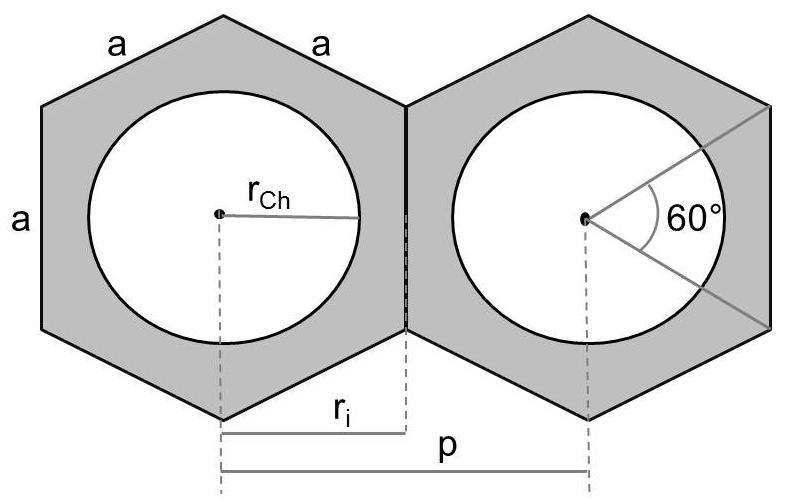
\includegraphics[width=.4\textwidth]{Bilder/MCP_hex.jpg}
			\caption{MCP honeycomb structure \cite{Diss_Neuland}.}
			\label{fig:MCPhex} % Ref. Maike Diss
		\end{figure}
		The number of channels $N$ of an MCP is its active area $A_{act}$ divided by the area of one channel $A_{hex}$. The MCP has a honeycomb like structure (Fig.\,\ref{fig:MCPhex}). Thus, the area of one channel is the area of a hexagon:
		\begin{equation}
			N = \frac{A_{act}}{A_{hex}} = \frac{2\cdot\pi r^2_{act}}{\sqrt{3}p^2}
		\end{equation}
		$r_{act}$ is the radius of the active area of the MCP which is for our MCPs 8\,\si{\milli\meter} and p is the distance between the centres of two channels which is 6\,\si{\micro\meter}. This results in $1.6\cdot10^6$ channels.\\
		The resistance of a single channel is the resistance of the whole MCP plate $R_{MCP}$ times the number of channels $N$:
		\begin{equation}
			R_{ch} = R_{MCP}\cdot N
		\end{equation}
		Its resistance depends on the voltage applied over the plate. For a nominal voltage of 1000\,\si{\volt} $R_{MCP}$ is $\sim$70\,\si{\mega\ohm} resulting in channel resistance of about $10^{14}$\,\si{\ohm}.\\
		The MCPs consist of two different materials: the structure (grey) consists of a type of lead glass and the hole, which can be approximated with vacuum (white) (Fig.\ref{fig:MCPhex}). The area of the structure is equal to the area of the hexagon $A^{hex}_{ch}$ minus the area of the channel hole $A^{hole}_{ch}$. the capacitance of one channel $C_{ch}$ is:
		\begin{equation}
			C_{ch} = \frac{\epsilon_0  (\epsilon_r \cdot (A^{hex}_{ch} - A^{hole}_{ch})+ A^{hole}_{ch})}{l_{ch}}
		\end{equation}
		With $\epsilon_0$ the vacuum permittivity, $\epsilon_r$ the relative permittivity of lead glass and $l_{ch}$ the MCP thickness which is 0.3\,\si{\milli\meter}. The relative electric permittivity depends strong on the conditions under which the material is used for example under which voltage, frequency or temperature the MCPs are used. Furthermore, the manufacturer does not give details about the material characteristics as it is a company secret. In \cite{Diss_Neuland} is an analysis of different values for $\epsilon_r$ found in literature. These values are between 6 and 20. With these values, the resulting capacity is 5\,\si{\atto\farad} per channel. The dead time of a single MCP channel is the channel resistance $R_{ch}$ times the channel capacitance $C_{ch}$:
		\begin{equation}
			\tau = R_{ch}\cdot C_{ch}
		\end{equation}
		This results in a dead time of 500\,\si{\micro\second}. A typical waveform has a duration of about 100\,\si{\micro\second}. When an ion hits a channel, this channel would be blind for the next five waveforms. With $1.6\cdot10^6$ channels and assuming a uniform distribution of particles on the MCP surface, saturation is assumed at particle rates higher than $10^9$ particles/\si{\second}. % Do we really want to have this in? Because saturation really starts at 10^6 #/sec already due to other effects. If so, make at least a short remark to which effects.
		\begin{equation}
			U(t) = U_0\cdot(1- e^{-t/\tau})
		\end{equation}
		It is the time needed to recharge a single channel to approximately 63\% of its original charge. After $5\tau$ 99\% of the original charge is replenished. % Is only half true. Only under the assumption that all of the charge is extracted out of the MCP. May later further discussion and revision.
		
		
		
		% Atempt to calculate the acctual voltage drop of the MCP voltage in dependence of the count rate by taking into account the capacitorloading curve and the option of a possible paralyzability of the detector. To make that properly, a simulation would be necessary. Not relevant.
		
		\begin{comment}
			1 particle with tau as the dead time. Voltage of 1 channel when 1 particle hits the channel. We assume, that we do not get into saturation. At what particle rate does the voltage start to break down. When a particle hits the channel when the voltage is not full replenished, it empties the channel again.
			For a first approximation, wait for 5*tau until 99% of the voltage is recovered.
			Uch(tion) = U_0\cdot(1- e^{-tion/\tau}) % tion is the time when an ion triggers a signal.
			Assumption of this formula is that one ion empties the hole channel -> it extracts alls the current in the channel -> all ions should have the same amount of current = the same gain.
			
			1.6*10^6 particles/second -> 1#/6*10^-7 sec.
			
			ion arriving rate is constant and the ions distributed homogenious over the MCP plate
					
			tZero = countRate % time which resets your voltage to 0V of the channel.
			t_rate = 5*tau.
			Umcp = sum(Uch)/#Channels
			
			Temporal the count rate is much higher than the value averaged over 1 sec. -> The gain will drop within one spectrum but will recover to a certain amount until the next spectrum. This calculation looks at total paralyzability.
			
			See Simulations by Maike for the whole calculation -> also the gain drop is displayed there. Just summarize it here because it is interesting :) and it also gives sort of an approximation of the voltage drop.
			-> Weekend
			
		\end{comment}

		\textbf{Gain}\\
		% Check all variables, if it is consistent. Finish this chapter properly
		The following derivation is strongly based on the lecture notes of \cite{LecNot_Wurz2017}.	When an incoming particle hits the MCP channel wall there is a certain chance that it ejects an electron out of the channel wall. By applying an electric field $E$ over the MCP plate, this electron gets accelerated until it hits the opposite wall, where it ejects more electrons:
		\begin{equation}
			E = \frac{U_{MCP}}{l} = \frac{F}{q_0} = \frac{a m_e}{q_0}
		\end{equation}
		With $U_{MCP}$ the voltage applied over the MCP, $l$ the channel length, $F$ the force applied on the electron, $q_0$ the elementary charge and $m_e$ the mass of the electron. The acceleration of the electron is:		
		\begin{equation}
			a = \frac{U_{MCP}\cdot q_0}{l\cdot m_e}
		\end{equation}
		The distance $s$ an electron travels along the channel until it reaches the channel wall is:
		\begin{equation}
			s = \frac{1}{2}at^2 = \frac{U_{MCP}\cdot q_0\cdot t^2}{l\cdot m_e\cdot 2}
			\label{eq:DetGainChFlightDist}
		\end{equation}
		With $t$ the flight time of an electron until it hits the wall again. Assuming the initial velocity $v_{init}$ of the initial secondary electron is perpendicular to the channel wall, the flight distance until it hits the opposite channel wall is the channel diameter $d$. $t$ can be written as:
		\begin{equation}
			t = \frac{d}{v_{init}}
			\label{eq:DetGainChFlightTime}
		\end{equation}
		$v_{init}$ can be derived out of the electron's initial kinetic energy $U_{init}$:
		\begin{equation}
			U_{init} = \frac{1}{2}m_e v_{init}^2 \rightarrow v_{init} = \sqrt{\frac{2U_{init}}{m_e}}
			\label{eq:DetGainEkin}
		\end{equation}
		In inserting Eq.\eqref{eq:DetGainChFlightTime} and Eq.\eqref{eq:DetGainEkin} in Eq.\eqref{eq:DetGainChFlightDist} leads to:
		\begin{equation}
			s = \frac{q_0 \cdot U_{MCP}\cdot d^2}{l\cdot 4U_{init}}
			\label{eq:DetGainDistECh}
		\end{equation}
		The energy $U_c$ the electron gains during the flight time $t$ is:
		\begin{align}
			U_c = &q_0 Es = q_0\cdot \frac{U_{MCP}}{l}\cdot\frac{q_0\cdot U_{MCP}\cdot d^2}{l\cdot 4 U_{init}}\\
			= &q_0^2 \frac{U_{MCP}^2\cdot d^2}{l^2\cdot 4U_{init}}
		\end{align}
		The secondary electron emission coefficient $\delta$ is proportional to the square root of the energy $U_c$:
		\begin{equation}
			\delta = A\cdot \sqrt{U_c} = A\cdot \frac{q_0 U_{MCP}\cdot d}{2 \sqrt{U_{init}}\cdot l}
			\label{eq:DetGainDelta}
		\end{equation}
		With $A$ a fit constant. After $n$ collisions, the gain $G_{ch}$ of one channel is:
		\begin{equation}
			G_{ch} = \delta^{n} = \delta^{l/s}
			\label{eq:detGainDel}
		\end{equation}
		The number of collisions is the channel length $l$ divided by the distance an electron flies within the channel before it hits the channel wall and ejects more electrons $s$. Inserting now Eq.\eqref{eq:DetGainDelta} and Eq.\eqref{eq:DetGainDistECh} leads to:
		% alpha = l/d. Ref to [Wiza,1979] as the original formula is from him!!!
		\begin{equation}
			G_{ch} = \left(A\cdot\frac{q_0 U_{MCP} \cdot d}{2\sqrt{U_{init}}\cdot l}\right)^{\frac{4U_{init}}{q_0 U_{MCP}}\left(\frac{l}{d}\right)^2}
		\end{equation}
		By writing the channel length to diameter ratio $\frac{l}{d}$ as $\alpha$ and expressing the electrons initial energy $U_{init}$ in [eV], the equation turns into:
		\begin{equation}
			G_{ch} = \left(A\frac{U_{MCP}}{2\alpha\sqrt{U_{init}}}\right)^{\frac{4\cdot U_{init}\cdot\alpha^2}{U_{MCP}}}
		\end{equation}
		With $A$ in approximately 0.2 $\left(\frac{1}{eV}\right)^{1/2}$, % Ref. to Wiza
		$U_{MCP}$ in [eV], $\alpha$ is a dimensionless number and $U_{init}$ in the range of a few [eV].
		% cite here Wiza as done in Stefans diss

		
		% Explain as far as it is needed for the analysis of the detector results. Predictions, extrapolations on how the detector UMCP depends on UStack. Not quite clear which model we have to take for what reasons. Why a quadratic funtion at all. What other model will be more justified... Hmm... Have a look on how big this calculation is and may put it to the detector results in the experiments chapter.
		
		% Calculation of the detector current is part of the setup as there is a picture of the PS #2 and the cooresponding explanation of the measurement.
		% Include the circuit diagram of the detector. Explanation of the different components? Maybe? Change from diode to resistor? Reasons? (more robust but voltage over MCPs is not so easy to derive anymore)
		
		
		% Reference: Bieler Diss 2012, Wurz 2011, Scherer 1999, Meyer 2013 Data Analysis, Wells 2011
		
		
		% MCP detector. Gain calculation. How the detecotr works. Didn't do anything for further developement. But a lot of tests on the Galerie with not so a big output. There is about 1 graph where the gain curve is actually used. So this chapter is justified.
		% Dead time discussion is for nothing because it only shows that we do not reach the limit of our instrument. Only to show some nice calculation.
		
	
\begin{comment}
	
	Explain how a TOF works. Source, reflectron, detector.
	Explanation of the antechamber at the end after explaining the different parts.
	
	Detection efficiency Ionsource, MCP? -> y-Achse
	Mass Analyser, mass spectrometer. Most important formulas. dm/m = dt/t...
	Sensitivity
	Density enhancement -> explanation about closed and open source
	Sketch of the instrument
	Requirements: Power, mass, mass resolution,... (At the end or at the beginning. Introduction)
	
	
	Ionisationseffizienz/ Ionenproduktion der wichtigsten Gase. Detektionseffizienz hängt auch von Effizienz der MCPs ab... Erklären weshalb man die Achsenskalieruing braucht (entweder Counts oder die angepasste a.u. bei der Fläche und Counts/s für das Spektrum)
	
\end{comment}
		